\chapter{Background and Basics} % Main chapter title



\label{Background} 
%----------------------------------------------------------------------------------------
%	SECTION 1
%----------------------------------------------------------------------------------------
I often made the mistake to start talking about diffraction assuming the audience knows exactly what I mean. I'd like to rectify that here and introduce the concept and physics of \textit{diffraction} in the SEM. I wrote this chapter as an introduction to theory the first year PhD me would have liked to have read, assuming the wisdom of today. 

In this introductory chapter I will first lay out some key crystallography concepts as the Bravais lattice, indices notations and the reciprocal space. All these concepts will be illustrated by examples using the hexagonal lattice. In this way I can cover both the some basic physics concepts, introduce language and notations commonly used in this field but also evidence where some of the computations used in the later chapters come from. 


We cannot make a single dent in diffraction without a working knowledge of symmetry in crystallography, which is why I will take a few pages to explore \textit{crystal symmetry} and \textit{point group} analysis in Appendix~\ref{Chap:Symmetry}. Here I also will limit the examples to the wurtzite system to keep it relevant. On page~\pageref{sec:Wsymmetry}, I go over the defining symmetry operation of wurtzite space group derived in this Appendix. These operations are defining the relative positions of the atoms in the unit cell and  will be used in next chapter for computations of electron scattering factors.  

I will then talk about the interaction of electrons with the crystal lattice that gives rise to elastic coherent scattering along certain directions and touch on \textit{Bragg's law} and it's geometrical form, the \textit{Ewald sphere}. I will also talk about the interaction of the electrons with the unit cell, which affects the intensity of the diffracting beam along chosen direction through the parameter known as the \textit{scattering factor}. There are always these two conditions to take into account when figuring out the diffraction intensity along a certain direction. And both of these parameters (scattering angle from lattice plane and scattering factor) can have values for which the diffraction beam intensity vanishes.


\section{Primer}
But first things first. We need to define terms and notions that we've both seen before but maybe are not quite as within reach as they ought to be in order to comfortably embark on this journey.

\subsection{Crystal structure}
\label{Sec:crystalStruct}
At the atomic level many solids can be described as periodic and rigid arrangements of atoms. It is this periodicity that, as we will see, gives rise to diffraction phenomena which in turn allow us to observe and study very small features in solids. The \textit{periodic arrangements of atoms or molecules} also constitutes the loose definition of a \textit{crystal structure}.

The rigorous definition involves the mathematical construct of crystal \textit{lattice} which characterises its translational symmetry. Figure~\ref{Fig:motif} (b) shows an example of a lattice in 2D space (technically known as a \textit{net}). Every point is identical to any other point. When the lattice is populated uniformly by the same fixed structure, or motif, we generate the periodic arrangement we mentioned previously. We show in Fig.~\ref{Fig:motif}~(a) a $4\times4$ square motif which, when applied to every point in the 2D lattice, generates the tessellation or regular structure in Fig.~\ref{Fig:motif}~(c)\footnote{If you want to give 2D tessellation design a play here is a fun website: \href{http://gwydir.demon.co.uk/jo/tess/tess.htm}{link in pdf}.}. If the motif is a unit cell made up of atoms or molecules then we can talk about making up a crystal structure. 


%---------
\begin{figure}[!ht]
    \centering
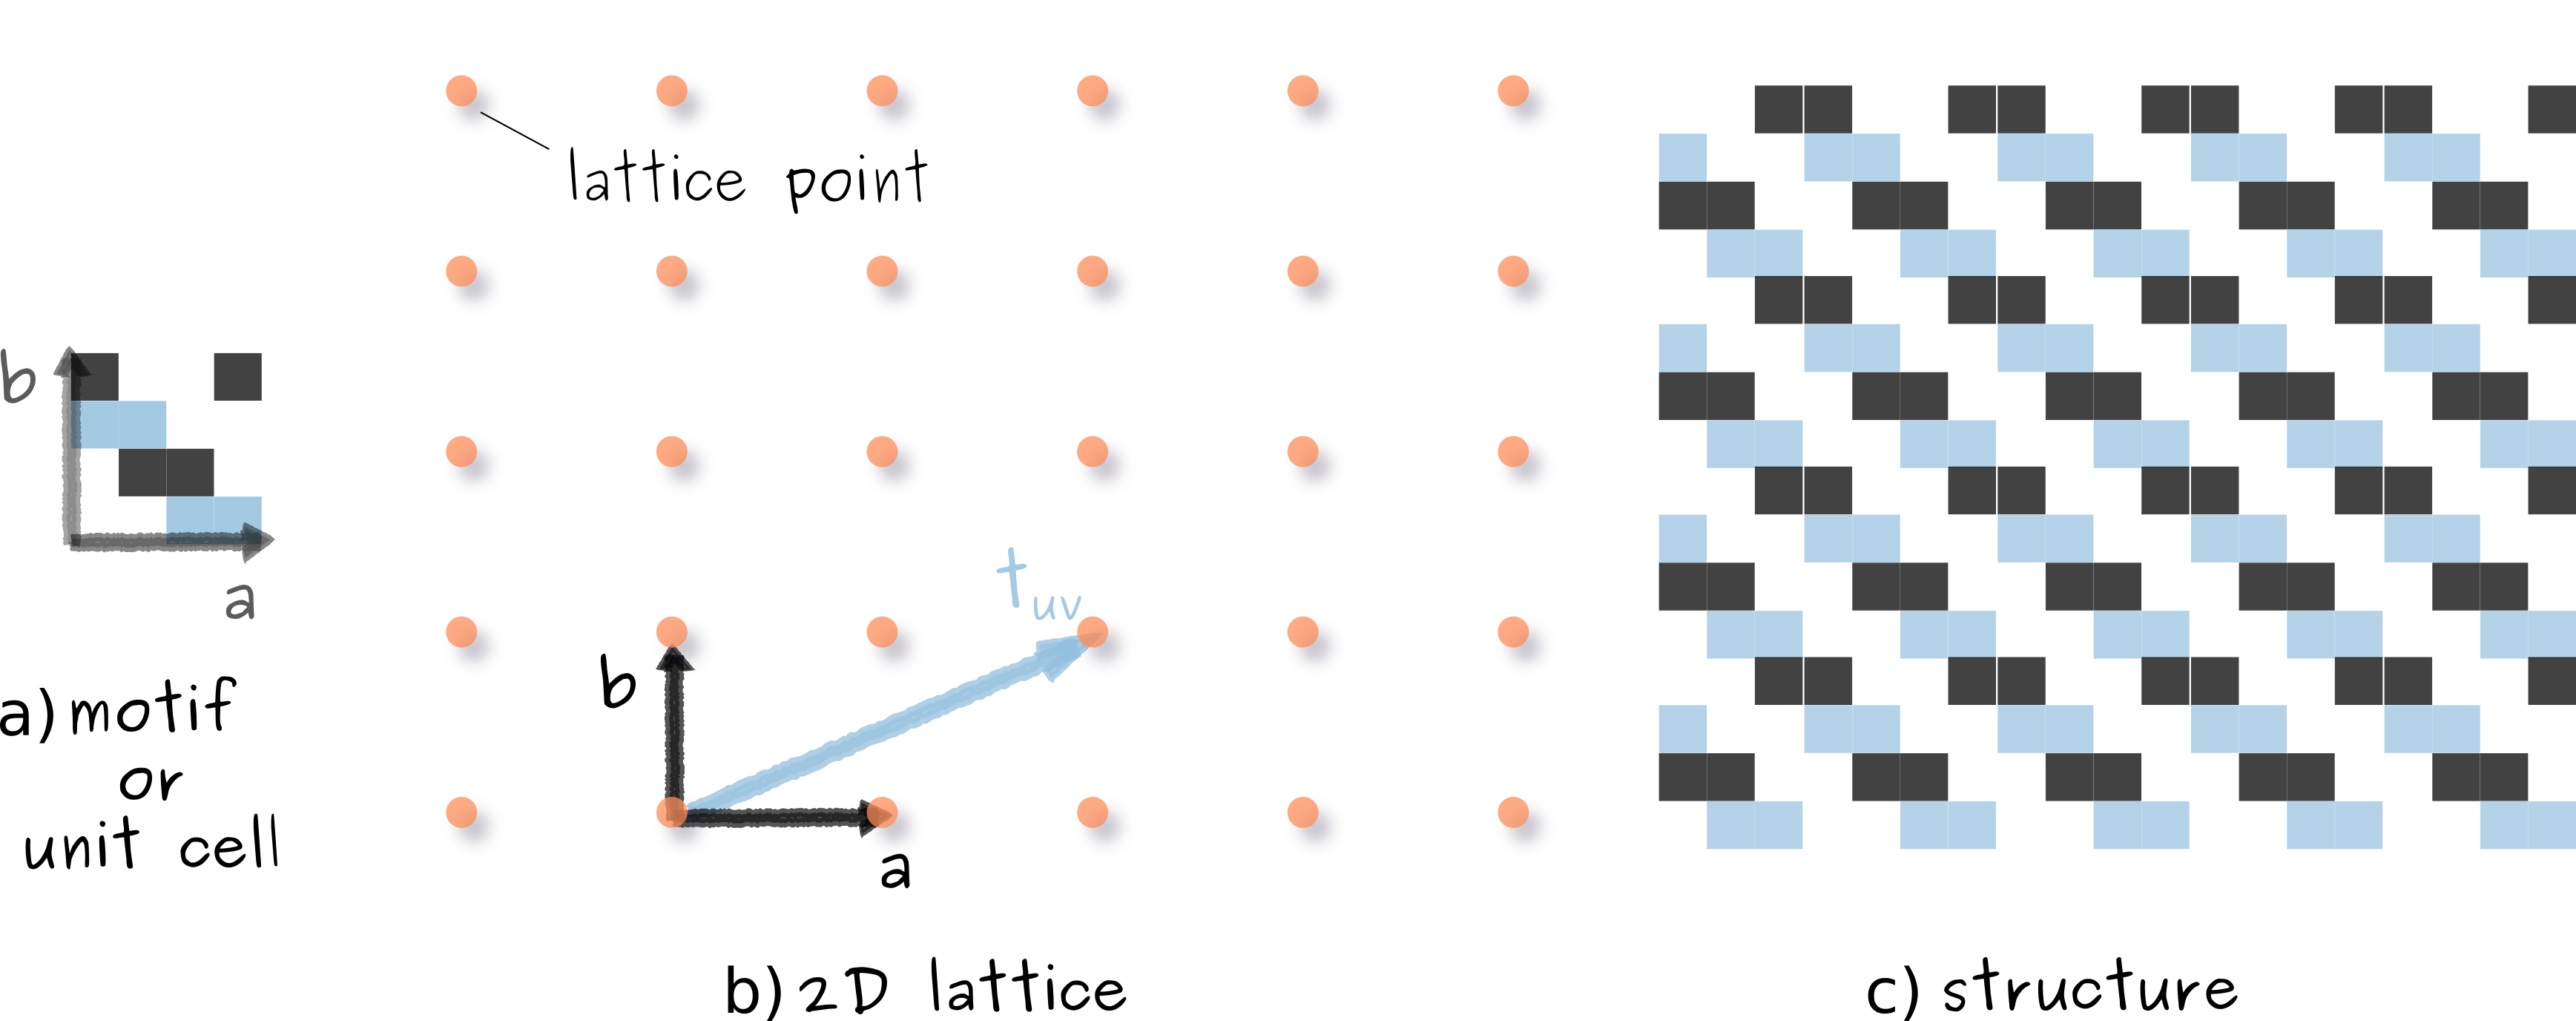
\includegraphics[width=0.9\linewidth]{Figures/motif.png}
\caption{A periodic structure (c) showing copies of a 2D motif (a) at every lattice point on a 2D lattice. The translation vector $t_{uv}$ moves the lattice to a position indistinguishable from the original one.}
\label{Fig:motif}
\end{figure}
%---------








\subsection{ \textbf{\textit{hP}} Bravais lattice and the hexagonal crystal system}


     
\label{Sect:spaceLattice}
There are as many lattices as there are possible regular arrangements of lattice points and there are as many possible arrangements as variety of crystal forms observed in nature. In the example above we placed the motifs such that its four corners coincide with four lattice points. In this case the motif maps exactly to one lattice point. In 3D space, we would have had the option to map a 3D motif on one, two or tree lattice points, defining lattices known as primitive ($P$), either body-centred ($I$) or base-centred ($C$), and face-centred ($F$), respectively. It is also easy to see that a motif with a very different shape will need a different arrangement of lattice points in order to cover the entire space neatly with no gaps or overlaps. We need, therefore, to unambiguously define both the lattice arrangement and the motif that define a crystal structure.   

A specific arrangement of lattice points displays a unique translational symmetry which, in turn, can be characterised by a set of \textit{basis vectors} usually denoted $\vb{a}, \vb{b}, \vb{c}$ for a 3D lattice. Fig.~\ref{Fig:motif} (b) shows the two basis vectors $\vb{a}, \vb{b}$ of the 2D lattice we used. We can think of them as having their origin in one of the corners of the motif structure and running along its edges. Together with the angle between them, the basis vectors can be used to define both the shape of the motif and lattice it can tessellate. We commonly define a unique 3D lattice by its lattice parameters $\{\mathsf{a}, b, c, \alpha, \beta, \gamma\}$ where $\mathsf{a}, b, c$ are the lengths of the vectors $\vb{a}, \vb{b}, \vb{c}$, $\alpha$ is the angle between $\vb{b}$ and $\vb{c}$, $\beta$ is the angle between $\vb{a}$ and $\vb{c}$ and $\gamma$ is the angle between $\vb{a}$ and $\vb{b}$, respectively. 

The volume described by the lattice parameters is known as the \textit{unit cell} of the lattice. While, for any given lattice, we can always find a \textit{primitive} unit cell, whose volume contains only one lattice point, in practice working with a high symmetry cell which reflects the point group symmetry of the crystal structure is preferred. We will talk more about point and translation symmetry as applied to crystallographic symmetry in Appendix~\ref{Chap:Symmetry} on page~\pageref{Chap:Symmetry}.

We can now also identify the position of any point on the lattice with the help of the basis vectors. Let us introduce the \textit{translation vector}, defined as the distance between any two points on the lattice. We can write it as $\mathbf{t}_{uv}=u\mathbf{a}+v\mathbf{b}$ in 2D (shown in Fig.~\ref{Fig:motif} (b)), and $\mathbf{t}_{uvw}=u\mathbf{a}+v\mathbf{b}+w\mathbf{c}$ in 3D, where $u, v, w$ are integers. Every point on an infinite lattice is equivalent to any other point, such that if one would be to move the structure by $\mathbf{t}_{uv}$ while we weren't looking, we would not be able to tell anything had changed when we looked back. This means that all lattice points are identical and we can choose any of them as the origin. Such that, the position of any lattice point is an integer linear combination of basis vectors independent on the chosen origin.

\vspace{0.4cm}

\noindent \begin{minipage}{0.5\linewidth}
If the lattice parameter values are chosen with no restriction, the resulting lattice has low symmetry. Conversely, let us select a 2D lattice with the two basis vectors equal in length, $|\vb{a}_1|=|\vb{a}_2|=\mathrm{a}$\footnotemark, and the angle $\gamma$ between them of 120\si{\degree}, as shown in Fig.~\ref{Fig:hex2dlattice}. It is easy to notice that rotating this lattice by 60\si{\degree} around a lattice point picked as origin would produce the same lattice. Another way of saying this is that the lattice is invariant under a $2\pi/6$ rotation and by definition \textit{hexagonal}. Notably, we could have chosen $\gamma$ to be 60\si{\degree} and we would have ended up with the exact same lattice. 

\end{minipage}\hspace{0.5cm}
\begin{minipage}{0.5\linewidth}
 \centering
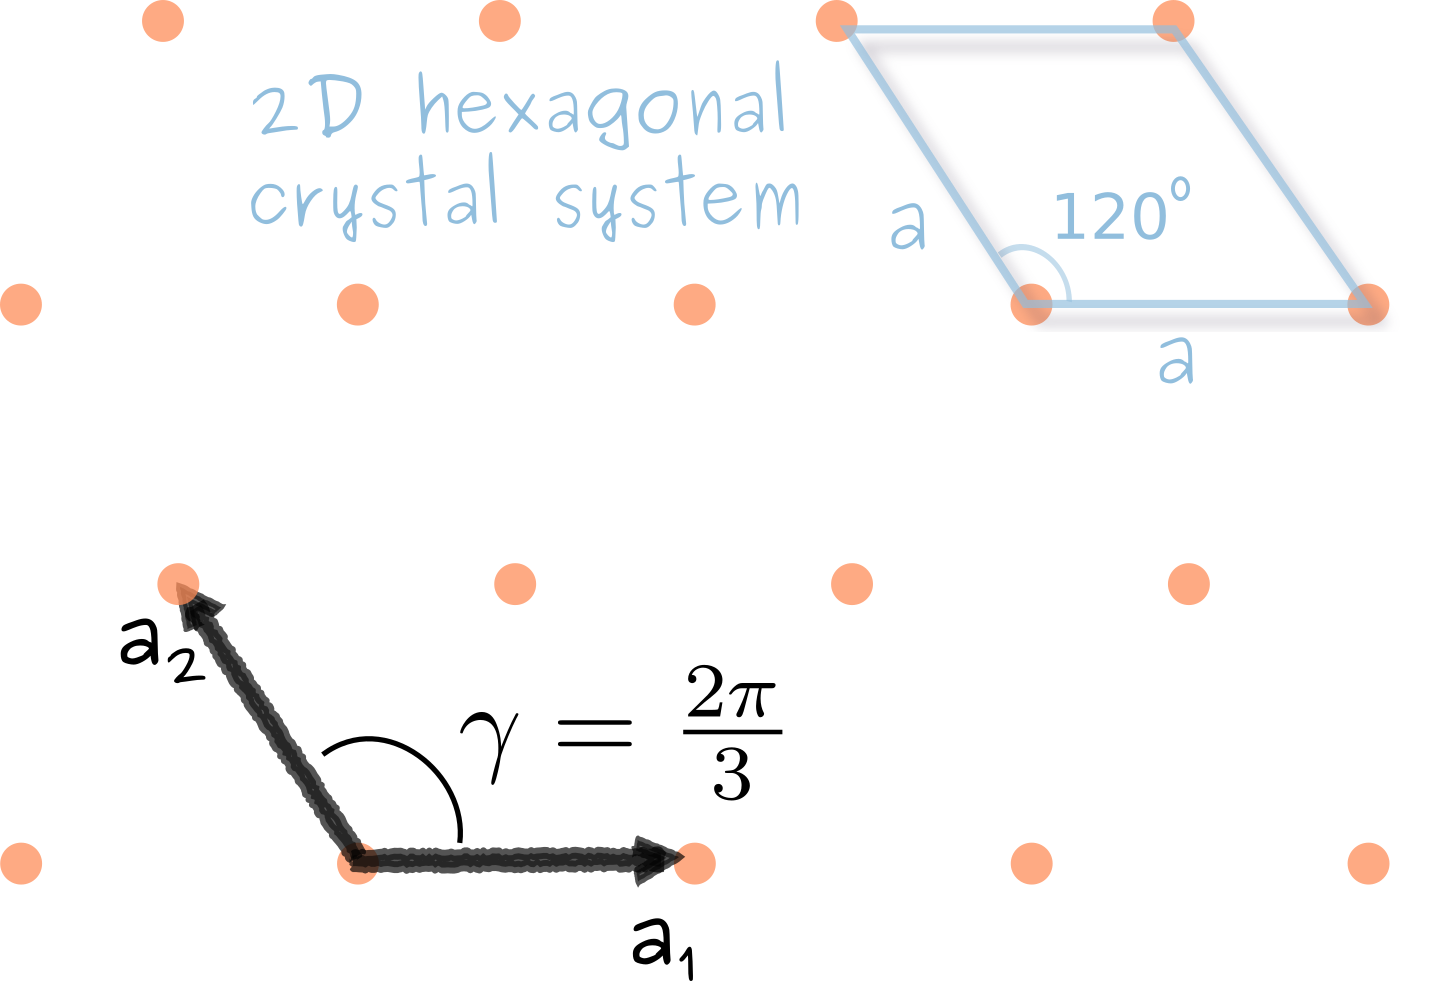
\includegraphics[width=1\linewidth]{Figures/hex2Dlattice.png}
\captionsetup{width=.8\linewidth}
\captionof{figure}{Hexagonal 2D lattice with basis vectors \{$\vb{a}_1$, $\vb{a}_2$, $\vb{c}$\}. The lattice parameters can be chosen to be \{$\mathrm{a}$,~$\mathrm{a}$,~$2\pi/3$\} or  \{$\mathrm{a}$,~$\mathrm{a}$,~$\pi/3$\}. }
\label{Fig:hex2dlattice}
\end{minipage}
 
\vspace{0.5cm}
\footnotetext{ A note about notation consistency. The general basis vectors of a lattice are \{$\vb{a}$, $\vb{b}$, $\vb{c}$\}. Whenever two or more vectors have the same magnitude we use the same letter and employ indices to differentiate between them such that the hexagonal lattice basis vectors are  \{$\vb{a}_1$, $\vb{a}_2$, $\vb{c}$\}.}

For every lattice with unique symmetry to be decorated with atoms, we talk about a specific \textit{crystal system}. We've seen that the hexagonal 2D crystal system can be described in at least two ways. Similarly, we can construct a $2\pi/6$ rotation invariant lattice in 3D by selecting the following special values for the lattice parameters:  $|\vb{a}|=|\vb{b}|$, $\alpha = \beta = 90\si{\degree}$ and $\gamma=120\si{\degree}$ as shown in Fig.~\ref{Fig:hex3lattice} (a). Here all we did was to add a $\vb{c}$ axis normal to the 2D hexagonal lattice and set it as the rotation axis. This is easy to see when comparing the 2D and 3D hexagonal crystal system.
 
We defined our unit cell as having the edges at lattice points but we did not yet specified which lattice points. It is convenient to opt for a unit cell that is simple and describes the point symmetry of the underlying lattice. It is also useful to work with a small volume and, in practice, the smallest cell that reflects the full symmetry of the system is used. When the unit cell is small enough such that it only contain one full lattice point, \ie primitive cell, it is denoted by $P$ as we have done in the choice of hexagonal unit cell shown in Fig.~\ref{Fig:hex3lattice} (b) where $h$ stands for hexagonal. Otherwise, the choice of unit cell is somewhat arbitrary, so much so that the Wigner-Seitz cell, which is centred on a lattice point and defined as the region of space closer to that lattice point than any other one, does not have edges aligned with lattice points. 


 
\begin{figure}[!htb]
\centering
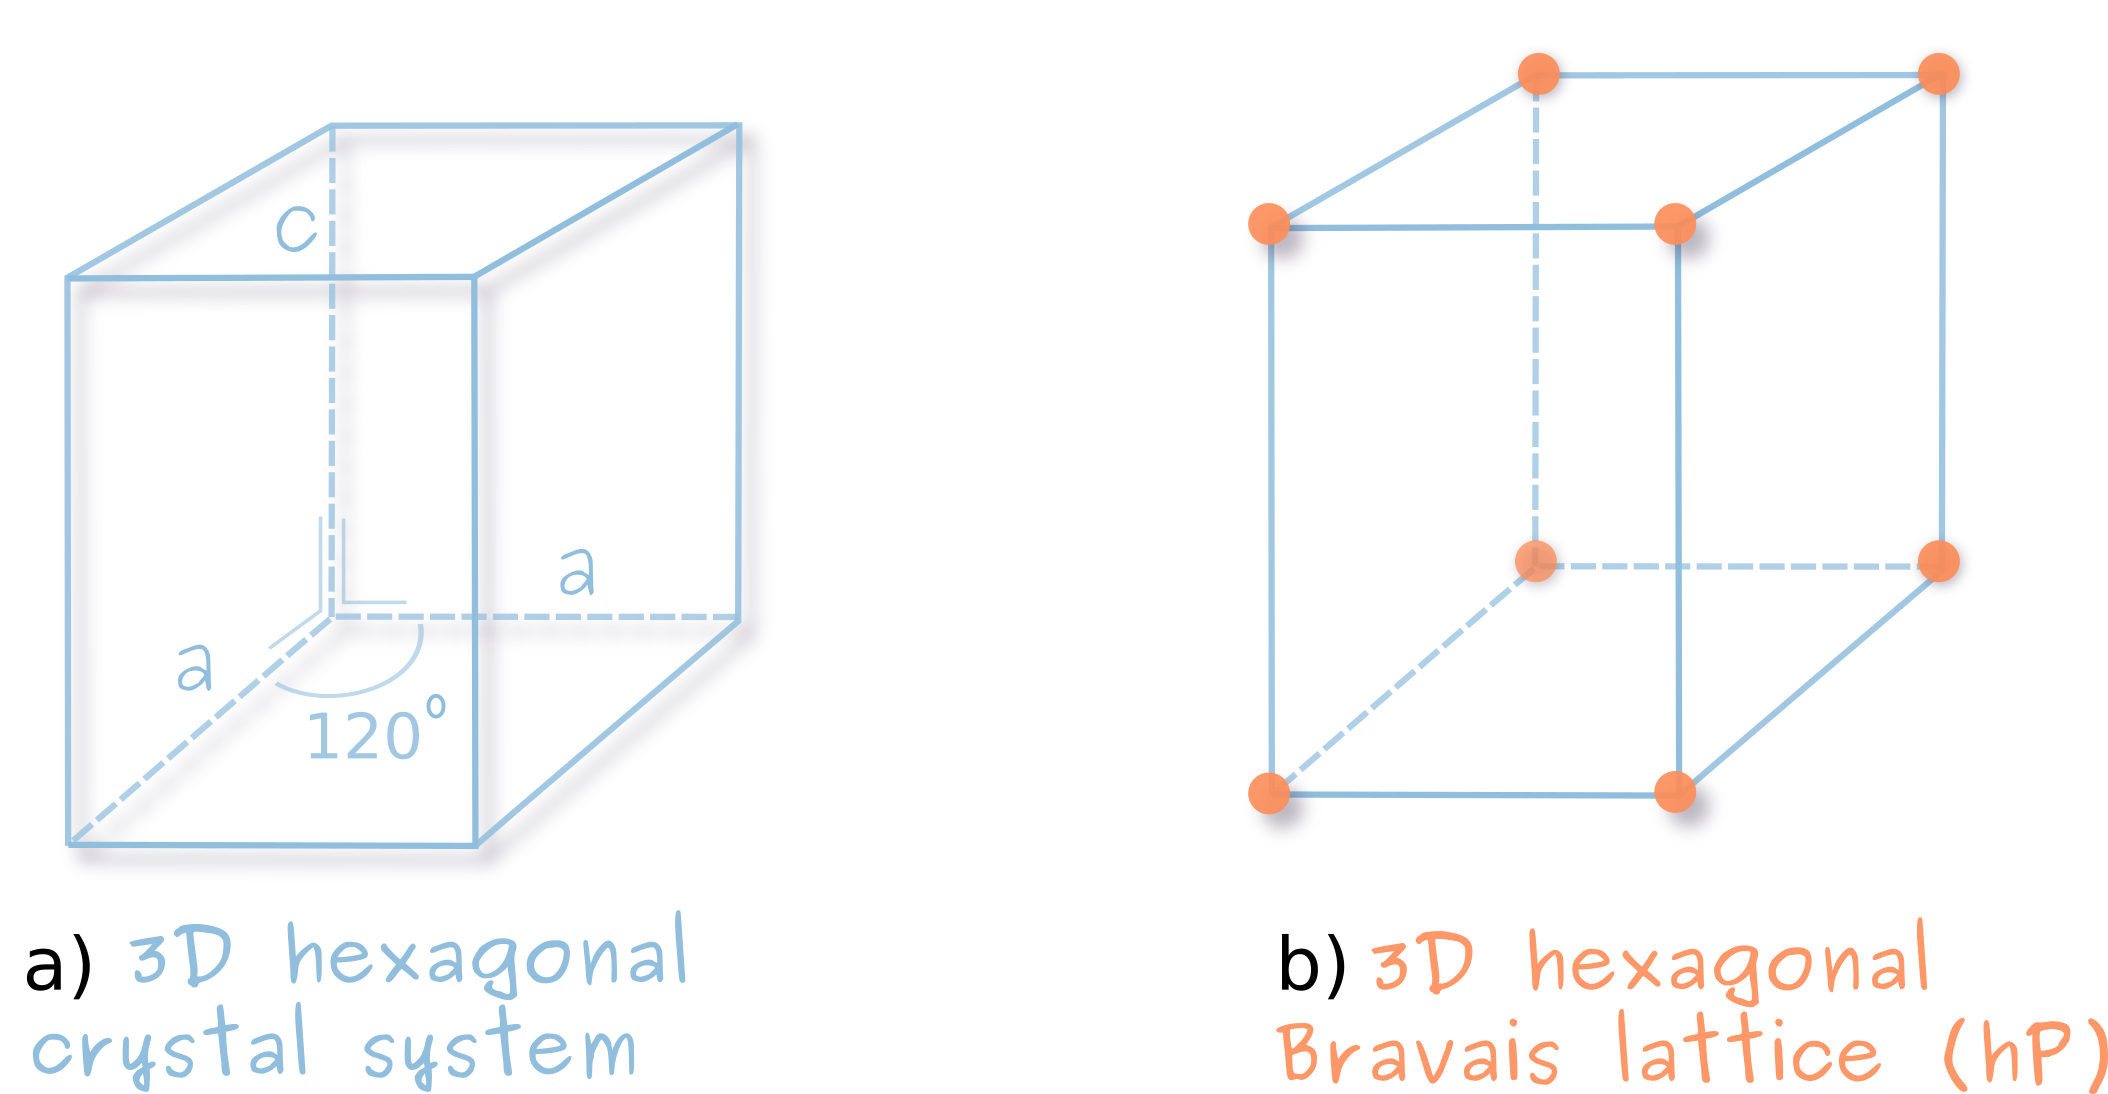
\includegraphics[width=0.7\linewidth]{Figures/hex3Dlattice.png}
\caption{3D hexagonal crystal system  with lattice parameters \{$a$, $a$, $c$, 90\si{\degree}, 90\si{\degree}, 120\si{\degree}\} (a) and the 3D hexagonal primitive lattice (b).  }
\label{Fig:hex3lattice}
\end{figure}


The same crystal system can be populated with lattice points in different manners such that it ends up describing different lattices. However, the number of choices of unique lattice points arrangements is limited to 5 for 2D lattices and 14 for 3D lattices. These unique lattice generators are known as \textit{Bravais}. The cubic crystal system ($c$), for instance, can be populated by a different number of lattice points: one to form the \textbf{p}rimitive cubic Bravais lattice ($cP$), two in the body centred lattice ($cI$) \footnote{ The label $I$ comes from the German word for body centred \textit{Innenzentriert}. } or three for the \textbf{f}ace centred one ($cF$). See ref.~\cite{Wolff85} for more information on lattice labels nomenclature. The hexagonal Bravais lattice ($h$) comes only in one type: primitive ($hP$), as shown in Fig.~\ref{Fig:hex3lattice}~(b).  

We can also write out now, from geometry, the volume of a primitive hexagonal lattice $\Omega_{hex}$ which will become useful later:
\begin{equation}
\label{eq:UnitCellVolume}
\Omega_{hex} = a^2 \sin{60 ^{\circ}} c
\end{equation}

With the notion of a hexagonal crystal system and its cell parameters well laid out, in the following section we will look at how we commonly label a certain plane or direction in this system.




\subsection{Lattice planes and directions in the hexagonal system}
\label{sec:latMB}

There are in fact two ways we can refer to a given plane or direction in a hexagonal crystal. The usual, or \textit{Miller} notation which applies to all the crystal systems, or the hexagonal symmetry friendly \textit{Miller-Bravais} indexing method. The first is defined by three indices while the latter by four. For planes indexing, going from the four index notation to the three index one means dropping the redundant third index. However, for directions notations things are slightly more involved.

\subsubsection{Miller indices}

Miller wrote and taught extensively about a way to label crystal planes in terms of their intercepts with the crystal reference axes. It was because of this and his choice of $h,k,l$ letters that the indexing method now bears his name: \textit{Miller indexing}. The method is beautiful in its simplicity: find the intercept with the three basis vectors, invert the intercepts, and last but not least reduce to smallest relative primes. One can also obtain all the equivalent planes belonging to the same family by even permutations of the indices $h,k,l$. For the hexagonal system the \hkl(hkl) indices correspond to the \{$\vb{a_1}$, $\vb{a_2}$, $\vb{c}$\} basis vectors.

\label{disc:millervector}
For directions, usually labelled \hkl[uvw], the process is simpler; find the coordinates in the crystal frame of the vector pointing in that direction and reduce them to smallest relative primes. It is this latter step which prompts us to raise an important observation. The Miller notation for direction does not carry vector length information and should not be used for finding length information. This might sound obvious, yet the temptation to understand direction \hkl[uvw] as vector $\vb{t}_{uvw}$ is significant. The difference between the two becomes more apparent in the hexagonal system.


While the Miller indices notation is tremendously helpful when looking at families of planes in a cubic system, its powers become limited when tackling lower crystal symmetry. For instance in a system with lower than cubic symmetry, the family of planes for a given \hkl(hkl) plane is no longer made up of \emph{all} possible permutations of the Miller indices $h$, $k$ and $l$.

\subsubsection{Miller-Bravais indices}
\label{subChap:MB indices}

The hexagonal system indexing is a very different story. Usually treated as a special case in itself, the hexagonal system can keep the permutation equivalence property of Miller indexes as long as an extra, redundant basis vector is added. The new set of basis vectors, \{$\mathbf{A_1},\mathbf{A_2}, \mathbf{A_3}, \mathbf{C} $\}, introduces 4-dimensional type vectors~\cite{Frank65} in what is called \textit{Miller-Bravais indexing}~\cite{Nicholas66}. This notation replaces the rhombic prism primitive unit cell with a hexagonal one  made up of three primitive hexagonal Bravais lattices ($hP$), as seen in Fig.~\ref{Fig:hexPrism}. We show here the three-vectors basis set together with the four-vector one.


Three of the Miller-Bravais basis vectors are the Miller basis vectors: $\mathbf{A_1}=\mathbf{a_1}$, $\mathbf{A_2}=\mathbf{a_2}$ and $\mathbf{C}=\mathbf{c}$. The extra basis vector is coplanar with the first two and, therefore, linearly dependent on them: 
\begin{equation}
\label{eq:a1a2a3}
\mathbf{A_3} = - (\mathbf{a_1} + \mathbf{a_2)}=- (\mathbf{A_1} + \mathbf{A_2)}. 
\end{equation}
A vector $\vb{p}$ in this system is defined as $\vb{p} = p_1\mathbf{A_1}+p_2\mathbf{A_2}+p'\mathbf{A_3}+p_3\,\mathbf{C}$. When coordinates \{$p_1, p_2, p_3, p'$\} are integers, $\vb{p}$ becomes the translation vector $\vb{t}$ which shows a common direction in the crystal system. If we take this a step further and reduce the coordinates to relative primes then we obtain the reduced vector $\vb{t}_{uvtw}$ where indices $u,v,t,w$ form the Miller-Bravais notation.

\vspace{0.5cm}
%-------------
\noindent \begin{minipage}{0.4\linewidth}
	\centering
\captionsetup{width=.9\linewidth}
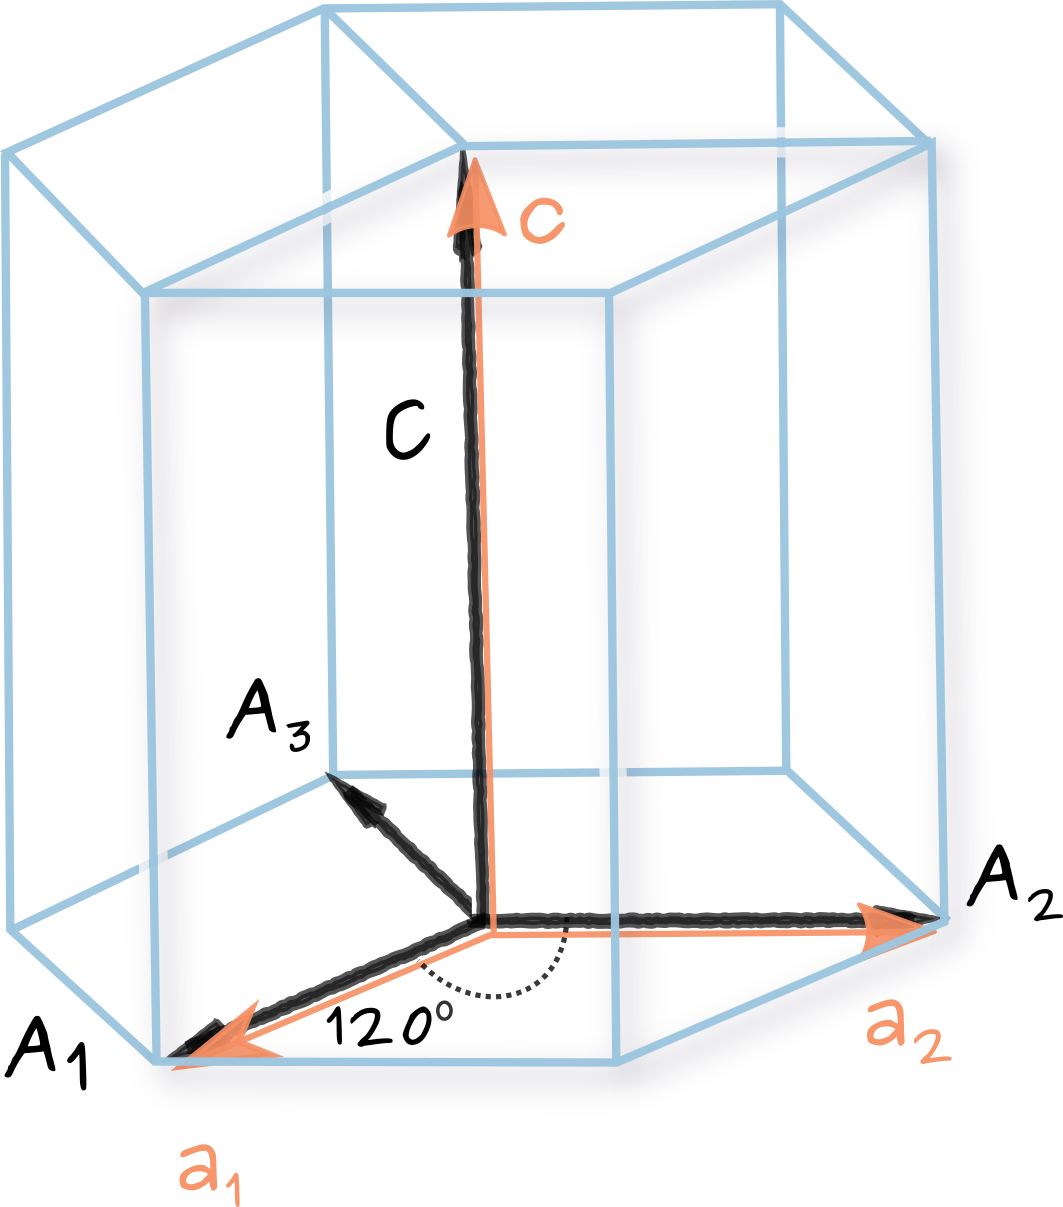
\includegraphics[width=0.75\linewidth]{Figures/Miller_Bravais.png}
\captionof{figure}{Hexagonal prism unit cell and the Miller-Bravais basis vectors \{$\mathbf{A}_1$,~$\mathbf{A}_2$,~$\mathbf{A}_3$,~$\mathbf{C}$\}. }
\label{Fig:hexPrism}
\end{minipage}
\begin{minipage}{0.6\linewidth}
    \centering
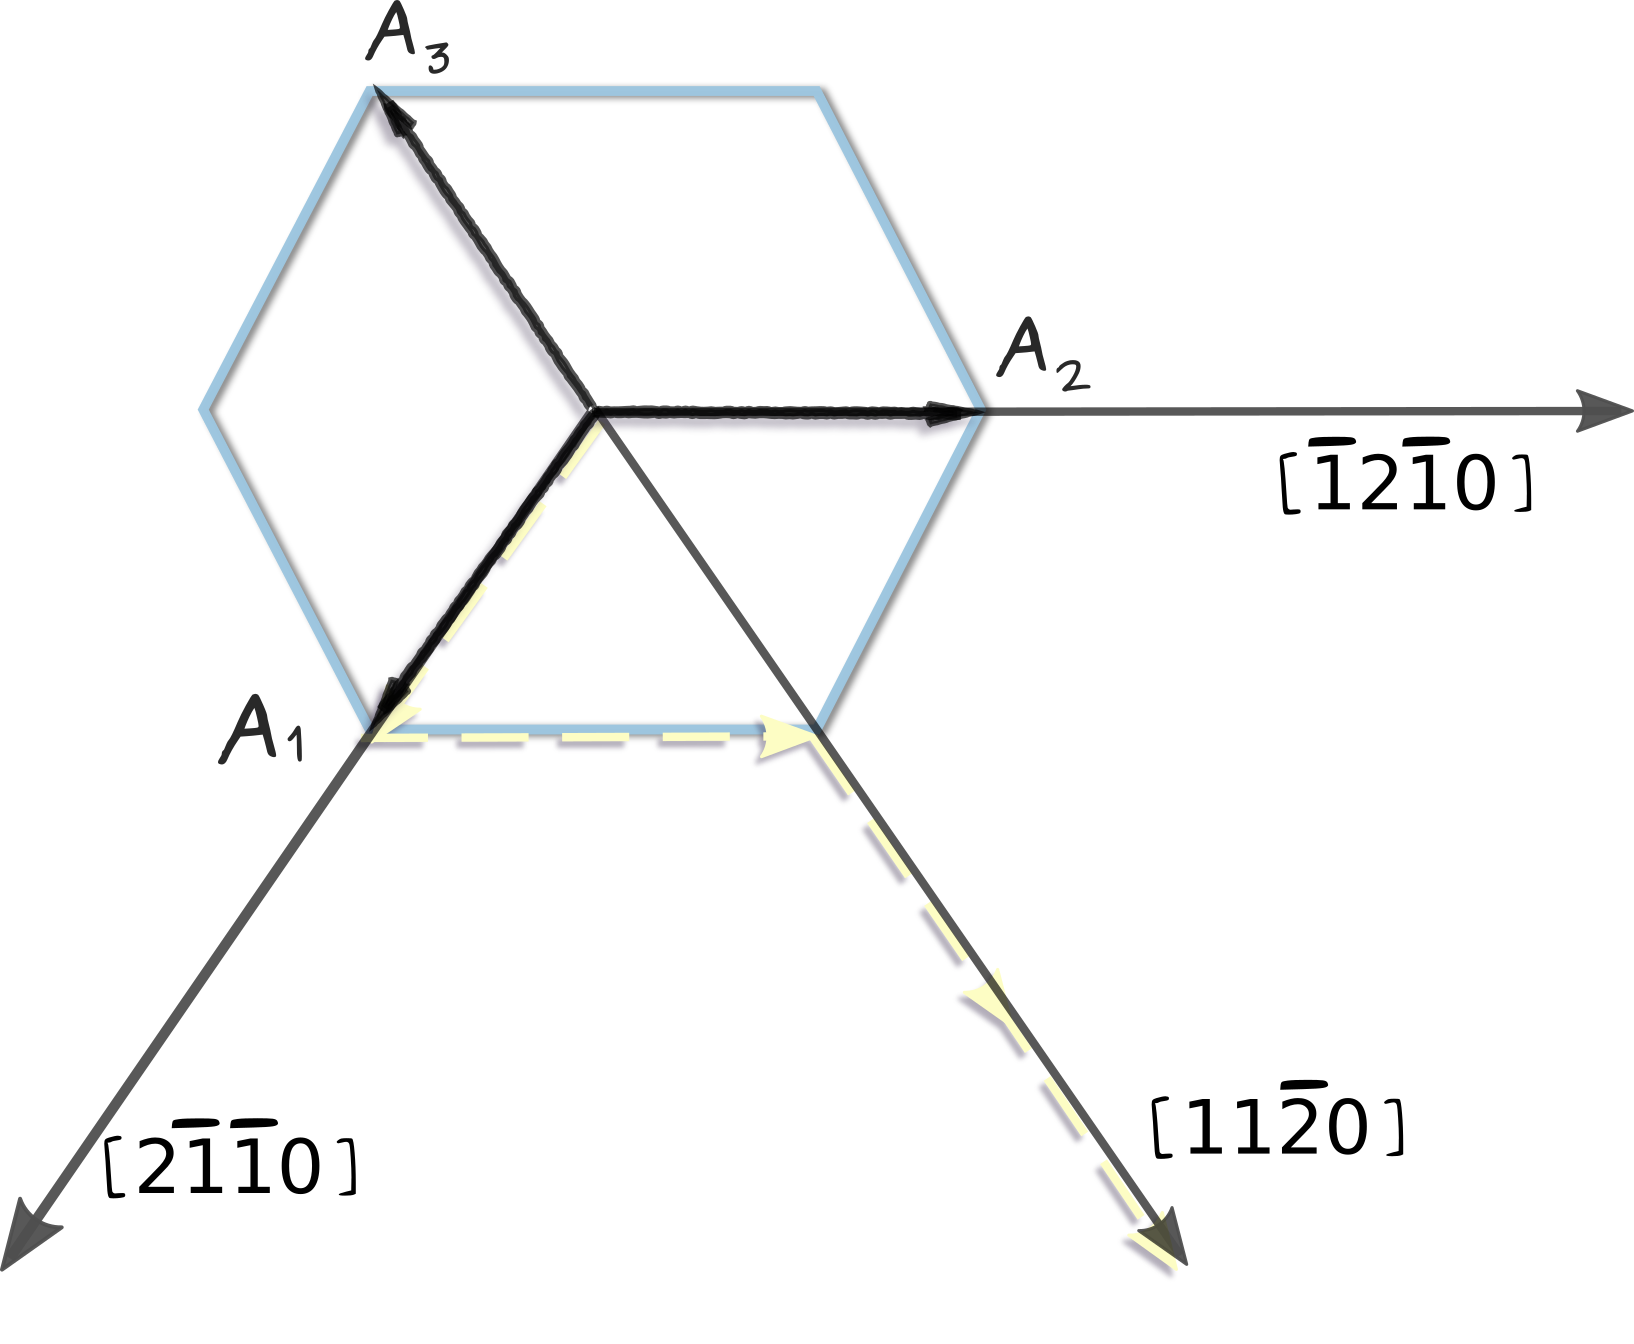
\includegraphics[width=0.65\linewidth]{Figures/fam_directions.png}
\captionof{figure}{Directions belonging to the \hkl<2-1-10> family. The yellow line shows the formation of the vector $\vb{t}_{\hkl[11-20]}$.  }
\label{Fig:directions}
\end{minipage}
%-------------

\vspace{0.3cm}

Directions in the four-index notations are of the form $u\mathbf{A_1}+v\mathbf{A_2}+t\mathbf{A_3}+w\,\mathbf{C}$ and written as \hkl[uvtw], where $u, v, t, w \in \mathbb{Z}$ and are relative primes. Comparing this expression to the same direction written with the three Miller basis vectors, $U\mathbf{a}+V\mathbf{b}+W\mathbf{c}$, yields the following true relations:

\begin{minipage}{0.3\linewidth}
\begin{equation*}
U=2u+v,
\end{equation*}
\end{minipage}%
\begin{minipage}{0.3\linewidth}
\begin{equation*}
V=2v+u,
\end{equation*}
\end{minipage}%
\begin{minipage}{0.3\linewidth}
\begin{equation}
W=w,
\end{equation}
\end{minipage}

\noindent and also
\begin{equation*}
t=-(u+v).
\end{equation*}

Because the first three basis vectors are not linearly independent, writing out their Miller-Bravais indices is somewhat awkward as seen in Fig.~\ref{Fig:directions}. The three coplanar vectors ensure that any given directions will have at least two non-zero components, and the $\mathbf{A}_i$ basis vectors themselves have three non-zero components. While the Miller direction vectors corresponding to the basis vectors directions have the same lengths as the basis vectors themselves, this is not the case in the Miller-Bravais notation, see vector $\vb{t}_{\hkl[11-20]}$. Nevertheless, we can find families of directions through the usual permutations which would not be possible using the Miller notation as we can see from Table~\ref{Table:MB_directions}. 

%--------
\begin{table}[!htb]
\caption{Some common directions in hexagonal system given in Miller and Miller-Bravais notation.}
\label{Table:MB_directions}
\centering
\begin{tabular}{ l c c }
\toprule
\tabhead{Family} &\tabhead{Miller-Bravais} &\tabhead{Miller}\\
\midrule
\multirow{4}{*}{\hkl<2-1-10>} & \hkl[2-1-10] & \hkl[100]\\
						 & \hkl[11-20] & \hkl[110]\\
                         & \hkl[-12-10] & \hkl[010]\\
                         & \hkl[-2110] & \hkl[-100]\\
\bottomrule
\end{tabular}%
\hspace{0.5cm}%
\begin{tabular}{ l c c }
\toprule
\tabhead{Family} &\tabhead{Miller-Bravais} &\tabhead{Miller}\\
\midrule
\emph{(cont...)}                 &               &        \\
\multirow{2}{*}{\vtop{\hbox{\strut \textit{\hkl<2-1-10>}}}}            
								& \hkl[-1-120] & \hkl[-1-10]\\
								& \hkl[1-210] & \hkl[0-10]\\
\midrule
\multirow{1}{*}{\hkl<0001>} & \hkl[0001] & \hkl[001]\\

\bottomrule
\end{tabular}
\end{table}
%--------

A plane description in the new basis set will be of the form \hkl(hkil) where $i$ can be found from $i=-(h+k)$ and, bearing no unique information, can be omitted from the notation: \hkl(hk.l). A family of planes is then given by the permutations of the first three Miller-Bravais indices including their negative values:

\begin{equation*}
\hkl{hkil} = \{\hkl(hkil), \hkl(ihkl), \hkl(kihl)\,\hkl(-h-k-il), \hkl(-i-h-kl), \hkl(-k-i-hl) \}.
\end{equation*}

Table~\ref{Table:MB_planes} shows a list of commonly used families of planes in a hexagonal system. A graphical representation of these planes is shown in Fig.~\ref{Fig:planes}. It is clear that the Miller indices are counterintuitive in this system and the Miller-Bravais notation is preferred. We also mention the polarity of each family of planes but we will postpone the explanation of polarity until the point group discussion on page~\pageref{subChap:pointGroup}.

%--------
\begin{table}[!htb]
\caption{Common planes in hexagonal system given in Miller and Miller-Bravais notation.}
\label{Table:MB_planes}
\centering
\begin{tabular}{ l c c }
\toprule
\tabhead{Family} &\tabhead{Miller-Bravais} &\tabhead{Miller}\\
\midrule
\multirow{6}{*}{\vtop{\hbox{\strut \textit{m-plane}}\hbox{\strut \textit{(non-polar)}}}} & \hkl(1-100) & \hkl(1-10)\\
						 & \hkl(01-10) & \hkl(010)\\
                         & \hkl(-1010) & \hkl(-100)\\
                         & \hkl(-1100) & \hkl(-110)\\
                         & \hkl(0-110) & \hkl(0-10)\\
                         & \hkl(10-10) & \hkl(100)\\
\midrule
\multirow{4}{*}{\vtop{\hbox{\strut \textit{a-plane}}\hbox{\strut \textit{(non-polar)}}}} & \hkl(11-20) & \hkl(110)\\
						 & \hkl(1-210) & \hkl(1-20)\\
                         & \hkl(-2110) & \hkl(-210)\\
                         & \hkl(-1-120) & \hkl(-1-10)\\
\bottomrule
\end{tabular}%
\hspace{0.5cm}%
\begin{tabular}{l c c }
\toprule
\tabhead{Family} &\tabhead{Miller-Bravais} &\tabhead{Miller}\\
\midrule
\multirow{3}{*}{\vtop{\hbox{\strut {\centering \emph{(cont...)}} }{\hbox{\strut \textit{a-plane}}\hbox{\strut \textit{(non-polar)}}}}}               &              &           \\
                         & \hkl(-12-10) & \hkl(-120)\\
                         & \hkl(2-1-10) & \hkl(2-10)\\
\midrule
\multirow{6}{*}{\vtop{\hbox{\strut \textit{r-plane}}\hbox{\strut \textit{(semi-polar)}}}} & \hkl(1-102) & \hkl(1-12)\\
						& \hkl(01-12) & \hkl(012)\\
                        & \hkl(10-12) & \hkl(102)\\
                        & \hkl(-1102) & \hkl(-112)\\
                        & \hkl(0-112) & \hkl(0-12)\\
                        & \hkl(-1012) & \hkl(-102)\\
\midrule                        
\multirow{1}{*}{\textit{c-plane} \textit{(polar)}} & \hkl(0001) & \hkl(001)\\
\bottomrule  
\end{tabular} 
\end{table}
%---------




%---------
\begin{figure}[!htb]
    \centering
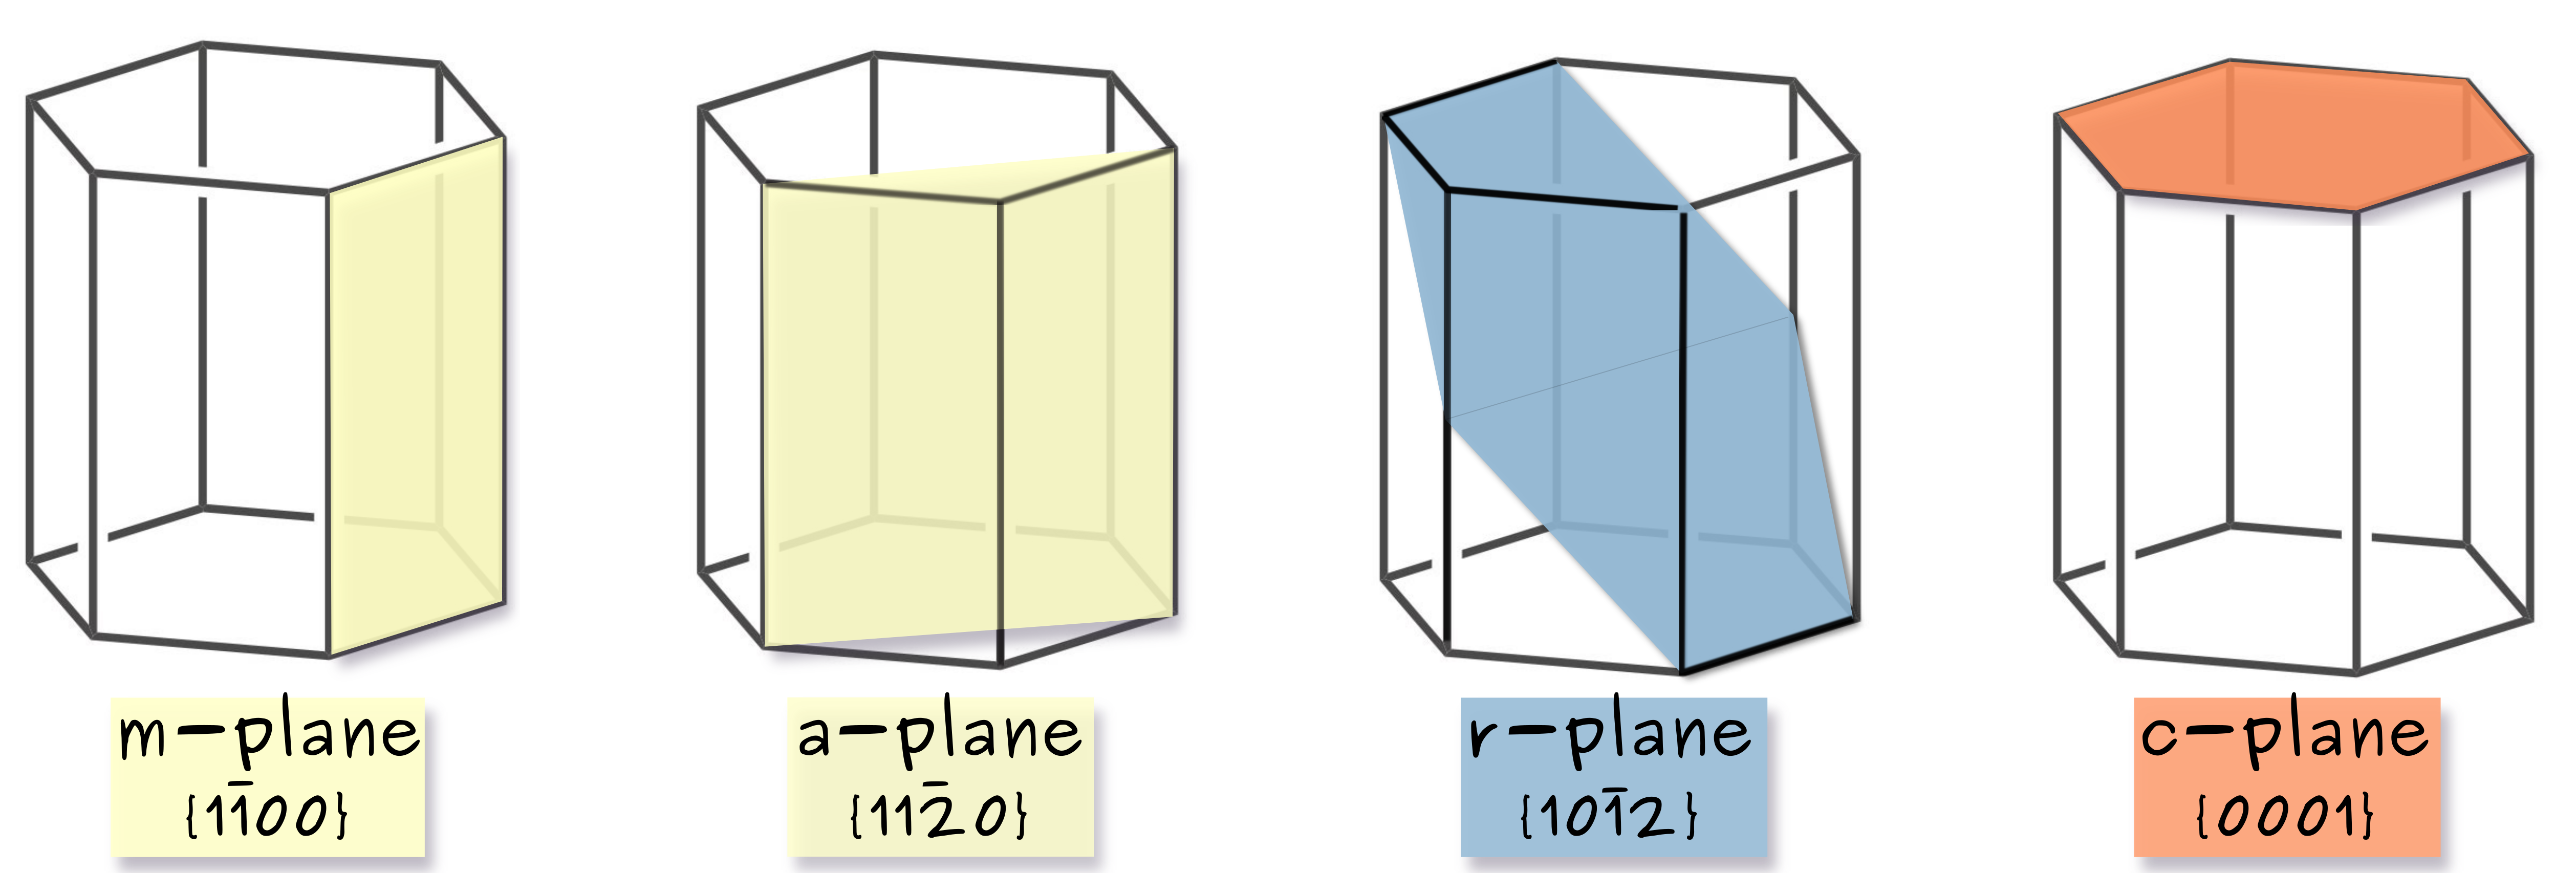
\includegraphics[width=0.85\linewidth]{Figures/hex_planes.png}
\caption{Common planes in hexagonal crystal structures.}
\label{Fig:planes}
\end{figure}
%---------
We can also expand the \textit{zone axis} definition, which tells us what planes, \hkl(hkl), belongs to direction or zone, \hkl[uvw], given in Miller indices as $hu + kv + lw = 0$ to the Miller-Bravais notation:
\begin{equation}
hu + kv + it+ lw = 0
\end{equation}

%---------
\subsection{The reciprocal space}
\label{sec:recMB}
We have all the Bravais lattice basis set mathematical framework of dealing with vectorial quantities in a crystal frame and yet we had to introduce Miller and Miller-Bravais indices which don't really fit in this vector space. This leads us to why crystallographers like to employ a very different vector space to ease computations, namely the \textit{reciprocal space}. So then, any vectorial quantities in a crystal (\ie position, direction, strain) can be defined in real space in terms of the basis vectors of its Bravais lattice, \{$\vb{a},\vb{b}, \vb{c}$\}, or, conversely, in the reciprocal space in terms of a new set of basis vectors defined such that the components of a direction vector are the Miller indices, \hkl(hkl), of the plane normal to that vector, \{$\vb{a^*},\vb{b^*}, \vb{c^*}$\}. To be on the safe side we usually denote vectors defined in the reciprocal space with $\vb{g}$ and the translation vector in reciprocal space by $\vb{g}_{hkl}$:
\begin{equation}
\label{eq:ghkl}
\vb{g}_{hkl} = h\vb{a^*}+k\vb{b^*}+l\vb{c^*}\,,
\end{equation}
where it must be true that:
\noindent\begin{minipage}{.2\linewidth}
\begin{equation*}
  \vb{a^*} = \frac{\vb{b} \times \vb{c}}{\Omega},
\end{equation*}
\end{minipage}%
\begin{minipage}{.2\linewidth}
\begin{equation*}
   \vb{b^*} = \frac{\vb{c} \times \vb{a}}{\Omega},
\end{equation*}
\end{minipage}%
\begin{minipage}{.285\linewidth}
\begin{equation}
\label{eq:recVectors}
  \vb{c^*} = \frac{\vb{a} \times \vb{b}}{\Omega}.
\end{equation}
\end{minipage}

\noindent with $\Omega$ being the volume of the unit cell, $\Omega=\vb{a}\cdot (\vb{b}\times \vb{c})$. Note, that both the dot and the cross products here must be generalised to non-Cartesian crystal frames forms and I show how to do that in next section, Section~\ref{chap:real+recAlg} on page~\pageref{chap:real+recAlg}. 


A few observations can be made straight away at this point:
\begin{itemize}
\item From dimensional analysis we can tell that the length of a reciprocal space vector, $|\vb{g}|$, will be measured in units of $<length^{-1}>$.
\item The reciprocal lattice parameters are going to be \{$a^*$, $b^*$, $c^*$, $\alpha$, $\beta$, $\gamma$\} with the same angle definition as before.
\item The dot product of a real space basis vector with its reciprocal space basis vector will yield zeros except for: $\vb{a}\cdot\vb{a}^*=\vb{b}\cdot\vb{b}^*=\vb{c}\cdot\vb{c}^*=1$ or:
\begin{equation}
\label{eq:adotastar}
\vb{a}_i\cdot\vb{a}^*_j=\delta_{ij}
\end{equation}

\end{itemize}


A less intuitive observation on this different perspective of the crystal space leads to some upside-down-world-like properties. If we consider a distance vector with components known in relation to a real space basis set, and want to transform it to another real space basis with basis vectors smaller in magnitude, in order to keep the magnitude of the vector we must increase its components values. This property of some vector to counter-vary the change in basis with an inverse change in their components we call \textit{contravariance}. If  for the same vector which tells a distance in real space, we do the same exercise in reciprocal space, we find that that a decrease of the basis set gives smaller vector components. This vector behaviour is called \textit{covariance}. The fact that the same vector can have opposite properties in these two different vector spaces tells us that the spaces themselves are reciprocal to each other.

You're welcome reader, you're now almost a crystallographer. The missing bit of information for being a full-fledged one is the Bragg diffraction condition which will be discussed on page~\pageref{Sec:Bragg}. It is because the Bragg's diffraction condition depends on the lattice plane orientation with respect to the incident beam and the distance between the set of planes under scrutiny, that having an easy way of find the normal to a plane \hkl(hkl) in the reciprocal space vector $\vb{g}_{hkl}$ becomes valuable in crystallography. Not least due to the vector $\vb{g}_{hkl}$ property of having its length equal to the inverse of the distance between the set of planes \hkl{hkl}:
\begin{equation}
\label{eq:dhkl}
d_{hkl} = \frac{1}{|\vb{g}_{hkl}|}.
\end{equation}



\subsubsection{The reciprocal hexagonal lattice}
\label{sec:recHex}
I will have to just state for now the form of reciprocal basis vectors for the hexagonal lattice. We will suspend the disbelief until page~\pageref{sec:crossProd} of \textit{Crystallographic Computations} sections, where I show how one could get the general form of the cross product.  Let us then assume that we can find the reciprocal lattice vectors \{$\vb{a^*_1}$, $\vb{a^*_2}$, $\vb{c^*}$\} to be in terms of the real space hexagonal lattice basis set, \{$\vb{a_1}$, $\vb{a_2}$, $\vb{c}$\} to be: 
\begin{equation}
\label{eq:3recvectors}
\vb{a^*_1}  = \frac{4}{3a^2} \vb{a_1} + \frac{2}{3a^2} \vb{a_2} ,\,\quad\quad\quad %
\vb{a^*_2}  = \frac{2}{3a^2} \vb{a_1} + \frac{4}{3a^2} \vb{a_2} ,\,\quad\quad\quad  %
\vb{c}^*  = \frac{1}{c^2} \vb{c}.
\end{equation}
Where the reciprocal hexagonal lattice translational vector is, from Eq.~\ref{eq:ghkl}:
\begin{equation}
^{hex}\vb{g}_{hkl} = h\vb{a^*_1}+k\vb{a^*_2}+l\vb{c^*}.
\end{equation}


%---------
\begin{figure}[!htb]
    \centering
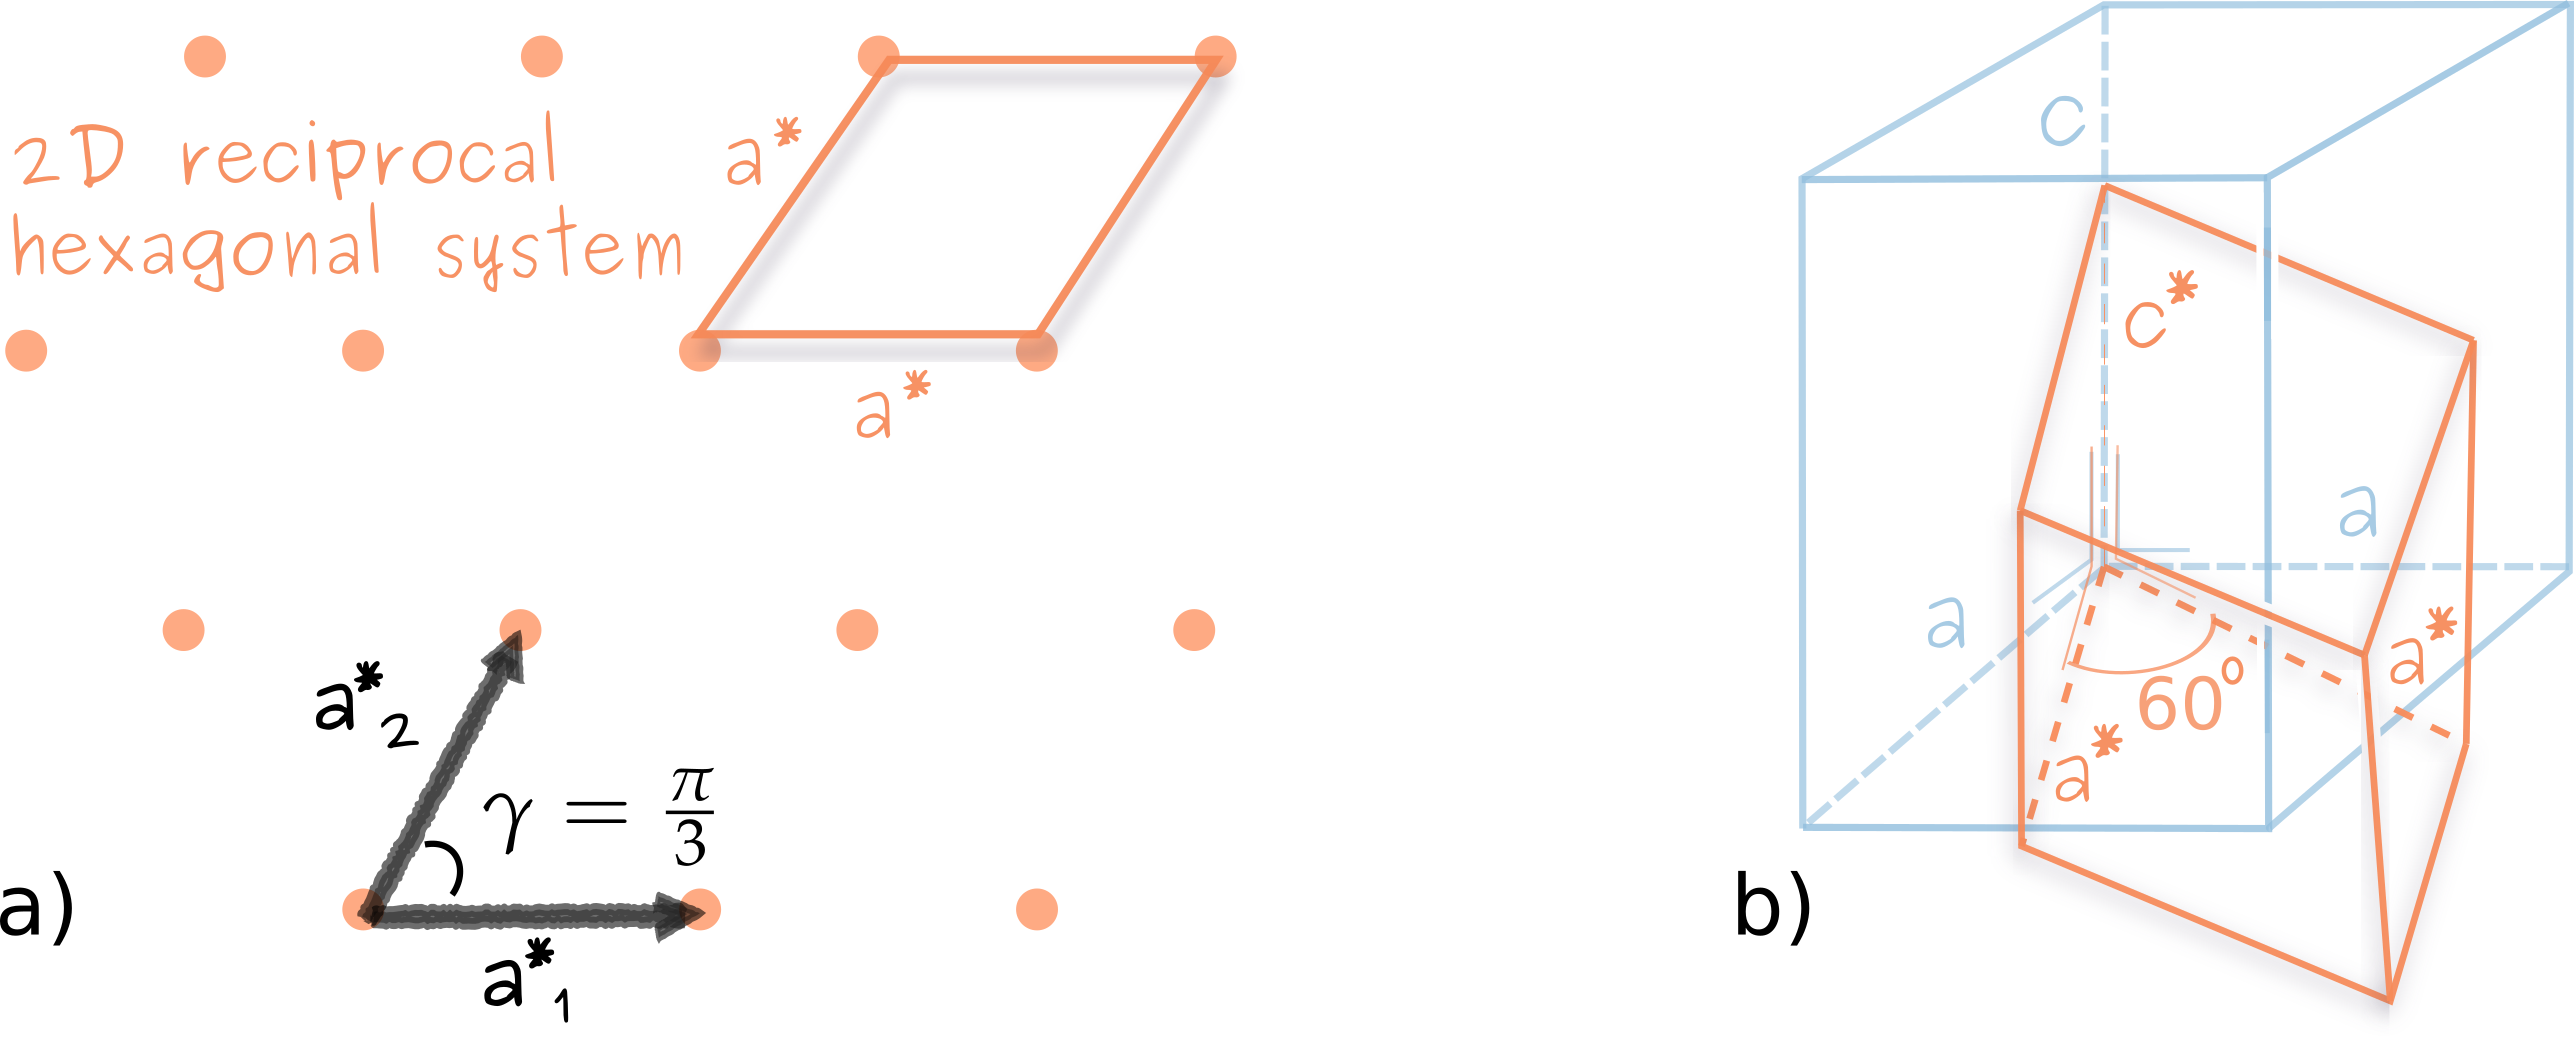
\includegraphics[width=.8\linewidth]{Figures/recHex.png}
\caption{Reciprocal 2D hexagonal lattice with basis vectors \{$\vb{a^*_1}$, $\vb{a^*_2}$\} and lattice parameters \{$a^*, a^*, 60\si{\degree}$\} (a) and the 3D reciprocal hexagonal crystal system with lattice parameters \{$a^*, a^*, c^*, 60\si{\degree}, 90\si{\degree}, 90\si{\degree}$\} over-imposed on the real space one while keeping the same origin (b).}
\label{Fig:recHex}
\end{figure}
%---------

Another noteworthy property of the reciprocal space is that the reciprocal crystal lattice must also be one of the 14 Bravais lattices. We have already seen in the discussion of Fig.~\ref{Fig:hex2dlattice} that the hexagonal lattice can be mapped by two lattice parameters sets. It turns out that the reciprocal hexagonal lattice has the same symmetry as the real space hexagonal lattice mapped by the other set of lattice parameters. Fig.~\ref{Fig:recHex}~(a) shows the reciprocal 2D lattice with parameters \{$a^*, a^*, 60\si{\degree}$\} which is comparable to Fig.~\ref{Fig:hex2dlattice}. The 3D reciprocal hexagonal system is the same hexagonal prism as in the real space with the lattice parameters \{$a^*, a^*, c^*, 60\si{\degree}, 90\si{\degree}, 90\si{\degree}$\} as can be seen in Fig.~\ref{Fig:recHex}~(b).



The first two vectors in both the real and reciprocal hexagonal system basis sets, \{$\vb{a_1}$, $\vb{a_2}$\} and \{$\vb{a^*_1}$, $\vb{a^*_2}$\}, respectively, do not align with each other as Fig.~\ref{Fig:recHex} indicates and  Fig.~\ref{Fig:recBasis} emphasises. This is the case for the 3-index notation. When the fourth index is added to form the reciprocal basis set \{$\vb{A^*_1}, \vb{A^*_2}, \vb{A^*_3}, \vb{C^*}$\} defining a lattice with parameters \{$A^*, A^*, A^*, C^*$, 120\si{\degree}, 120\si{\degree}, 120\si{\degree}, 90\si{\degree}, 90\si{\degree}, 90\si{\degree} \}  things get even more confusing. While the Miller-Bravais real and reciprocal co-planar hexagonal basis vectors, \{$\vb{A_i}$\} and \{$\vb{A^*_i}$\}, are parallel to each other, the two reciprocal basis sets, \{$\vb{a^*_i}$\} and \{$\vb{A^*_i}$\}, are not. Figure~\ref{Fig:recBasis} should make that somewhat more clear. 

\vspace{0.3cm}
\noindent \begin{minipage}{0.5\linewidth}
The four reciprocal basis vectors can be found in terms of the four real space basis vector to be:
\begin{align*}
\vb{A^*_1} & =\frac{2}{3a^2}\vb{a}_1, \, \quad \vb{A^*_2}=\frac{2}{3a^2}\vb{a}_2 
\end{align*}%
\vspace{-1cm}%
\begin{align}
\label{eq:4recvectors}
\vb{A^*_3} & =\frac{2}{3a^2}\vb{a}_3, \, \quad \vb{C^*}=\frac{1}{c^2}\vb{c}.
\end{align}
Where the four index reciprocal space translation vector is:%
\vspace{-0.5cm}%
\begin{equation*}
^{hex}\vb{g}_{hkil} = h\vb{A^*_1}+k\vb{A^*_2}+ i\vb{A^*_3} +l\vb{C^*}= \,\, ^{hex}\vb{g}_{hkl} \,.
\end{equation*}
\end{minipage}%
\begin{minipage}{0.57\linewidth}
%---------
\centering
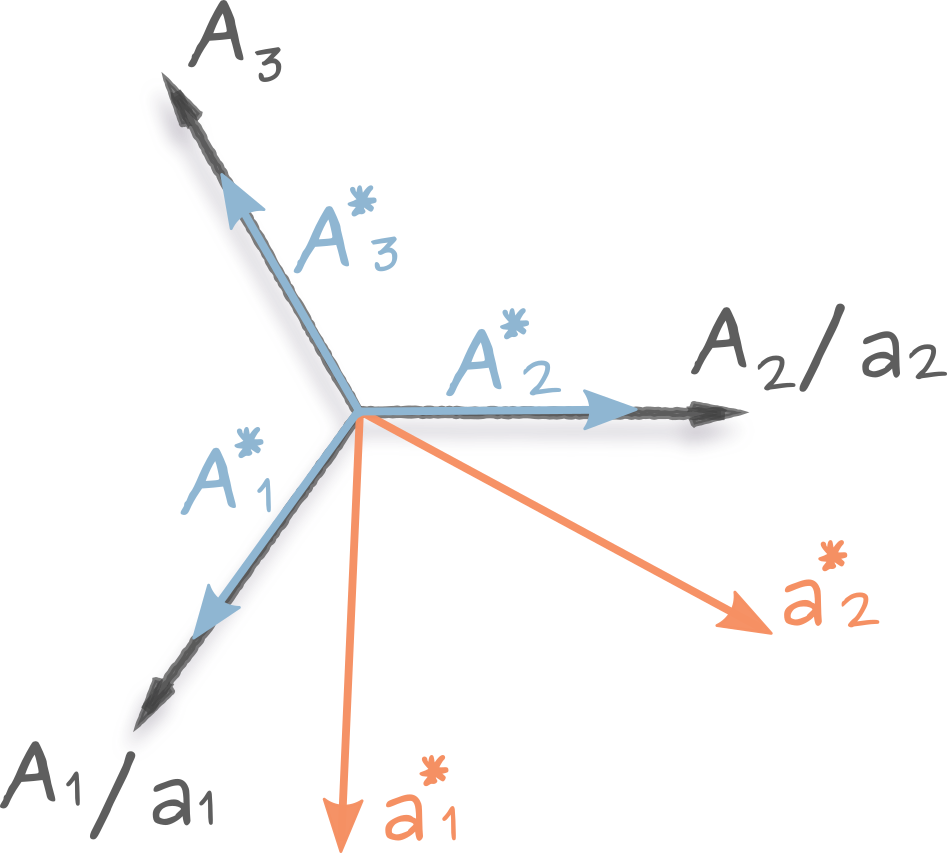
\includegraphics[width=.6\linewidth]{Figures/Miller_Bravais_rec.png}
\captionof{figure}{Relationship between real and reciprocal space hexagonal system basis sets. }
\label{Fig:recBasis}
%---------
\end{minipage}
%\vspace{0.3cm}

\label{say:moreDense}
The crystallographer must always be extra careful if using both notations. The two reciprocal basis vectors notations are not even describing exactly the same lattice. A closer inspection of Eq.~\ref{eq:3recvectors} and Eq.~\ref{eq:4recvectors}, tells us that the four-index reciprocal lattice is three times more dense than the three-index reciprocal one. Nevertheless, all the discussion about Miller-Bravais index notation still hold, \ie Eq.~\ref{eq:a1a2a3} is still valid, and the reciprocal space properties, including Eq.~\ref{eq:adotastar}, still apply. 

We will explore, in more depth, crystallographic computations in the hexagonal system, both in the real and the reciprocal space in Section~\ref{chap:real+recAlg} on page~\pageref{chap:real+recAlg}.

%
\subsection{Wavefunction as physical observable}
\label{sec:wave}
In the language of quantum mechanics, physical quantities are described via operators. The allowed values of the physical quantities are then eigenvalues of these operators. One must find the eigenfunctions of the corresponding operator in order to compute the value of a certain physical observable (\ie one must solve the equation $\hat{f}\ket{\Psi}=f\ket{\Psi}$).

For a free particle the momentum operator is $\hat{p}=i\hbar\grad$ where $\hbar$ is the reduced Planck's constant ($\hbar = h/2\pi$). The eigenvalues $\vb{p}$ and eigenfunctions $\ket{\Psi}$ of the momentum operator are defined by the equation:

\begin{equation*}
-i\hbar\grad \ket{\Psi}=\vb{p}\ket{\Psi}.
\end{equation*}
Which has solutions of the form:
\begin{equation*}
\Psi(\vb{r})=C e^{\frac{i}{\hbar}\vb{p}\vdot\vb{r}},
\end{equation*}
where $C$ is a normalisation constant.  
We can now use Louis de Broglie's relationship to relate momentum $p$ of a particle to a wavelength $\lambda$: $\lambda = h/p$. If the wave number $k$ is introduced, $k=1/\lambda$, then we can write in vector form $\vb{p}=h\vb{k}$.\footnote{ It is a consequence of the de Broglie formula that the momentum space is equivalent to the reciprocal space, apart from a scaling factor $h$.} Using this we can rewrite the wave function of a particle as a linear superposition of momentum eigenfunctions:
\begin{equation}
\label{eq:psi}
\Psi(\vb{r})=\sum_{\vb{k}} \psi_{\vb{k}} e^{2 \pi i \vb{k}\vdot\vb{r}},
\end{equation}
where the $C$ has been absorbed into the coefficients $\psi_\mathbf{k}$.

We will see in the next chapter that this expansion of the wave function in terms of plane waves makes the foundation of electron diffraction modelling. 

\pagebreak

%
\subsection{Plane waves}
\label{sec:planeWave}
Let us explore further the equation~\ref{eq:psi} above where $\mathbf{k}$ is the wave vector denoting the direction of travel of the wave and $\mathbf{r}$ is the position vector a point $P$ (see Fig.~\ref{Fig:planeWaves}).
\def\symbola{a}
Applying dimensional analysis for the exponent, one can show that, if the position vector $\mathbf{r}$ has components \{$r_1, r_2, r_3$\} with respect to the real space basis vectors \{$\vb{a}, \vb{b}, \vb{c}$\}:

\begin{equation*}
\mathbf{r} = r_1 \vb{a}  + r_2 \vb{b}  + r_3 \vb{c} ,
\end{equation*}
then the components of the wave vector $\mathbf{k}$ must be given with respect to the reciprocal basis vectors and, therefore, $\mathbf{k}$ must be a reciprocal space vector:
\begin{equation*}
\mathbf{k} = k_1 \mathbf{a^*} + k_2 \mathbf{b^*} + k_3 \mathbf{c^*}.
\end{equation*}

We will use this opportunity to quickly introduce a useful shorthand notation that allows crystallographers to be economic with their symbols. For this we have to slightly adjust the basis vector notation \footnote{ Another note on basis vector notation. Unfortunately, the letter $\vb{a}$ is overused in crystallography and can bear different meanings. Here we are using $\vb{a}_i$ to denote one component from a generic basis set in which all vectors are labelled with the same symbol but different subscripts. Real space basis in this notation is \{$\vb{a}_i, i \in (1, 2, 3)$\} and reciprocal space basis vectors are \{$\vb{a^*}_i, i \in (1, 2, 3)$\}.}:

\begin{equation*}
\mathbf{r}= r_1\vb{a_1} +r_2\vb{a_2}+r_3\vb{a_3}=\sum_{i=1}^3r_i \vb{a}_i\equiv r_i \vb{a}_i
\end{equation*}
\label{par:Einstein}
Since most of crystallography happens in 3D space we will always assume that the sum goes from $i=1$ to $i=3$ even when the limits are not written and the sum symbol, $\sum \,$, is dropped altogether. This is known as the \textit{Einstein summation convention} and its rule is that summation is implied over every pair of subscripts which appears on the same side of the equation. Using the Einstein summation convention the dot product $\mathbf{k} \cdot \mathbf{r}$ can be written as:
\begin{equation*}
\mathbf{k} \cdot \mathbf{r} = (k_i \mathbf{a_i^*})\cdot (r_i \mathbf{a_i}) = k_i r_j \delta_{ij} = k_i r_i,
\end{equation*}
where we made use of the definition of the reciprocal lattice: $\mathbf{a}_i\cdot \mathbf{a^*}_j=\delta_{ij}$.


\vspace{0.3cm}
\noindent \begin{minipage}{0.6\textwidth}
If we now ask the question of where in the real space is the wave going to have constant phase we can easily spot the required condition to be:
\begin{multline*}
\mathbf{k} \cdot \mathbf{r} = k_1 r_1 + k_2 r_2 + k_3 r_3 = \textrm{const.} , \\
\forall \, \mathbf{r} = r_1 \mathbf{a_1} + r_2 \mathbf{a_2} + r_3 \mathbf{a_3}
\end{multline*}
Which looks a lot like the equation of a plane:%
$$\mathbf{k}(\mathbf{r}-\mathbf{r_0}) = 0 $$
where $\mathbf{r_0}$ is the position vector of the origin of the wave vector $\mathbf{k}$ in the real space as shown in the figure to the right. The distance between consecutive planes of same phase values will be given by $\lambda = 1/|\mathbf{k}|$.

\end{minipage}
\begin{minipage}{0.4\textwidth}
\centering
\captionsetup{width=.7\linewidth}
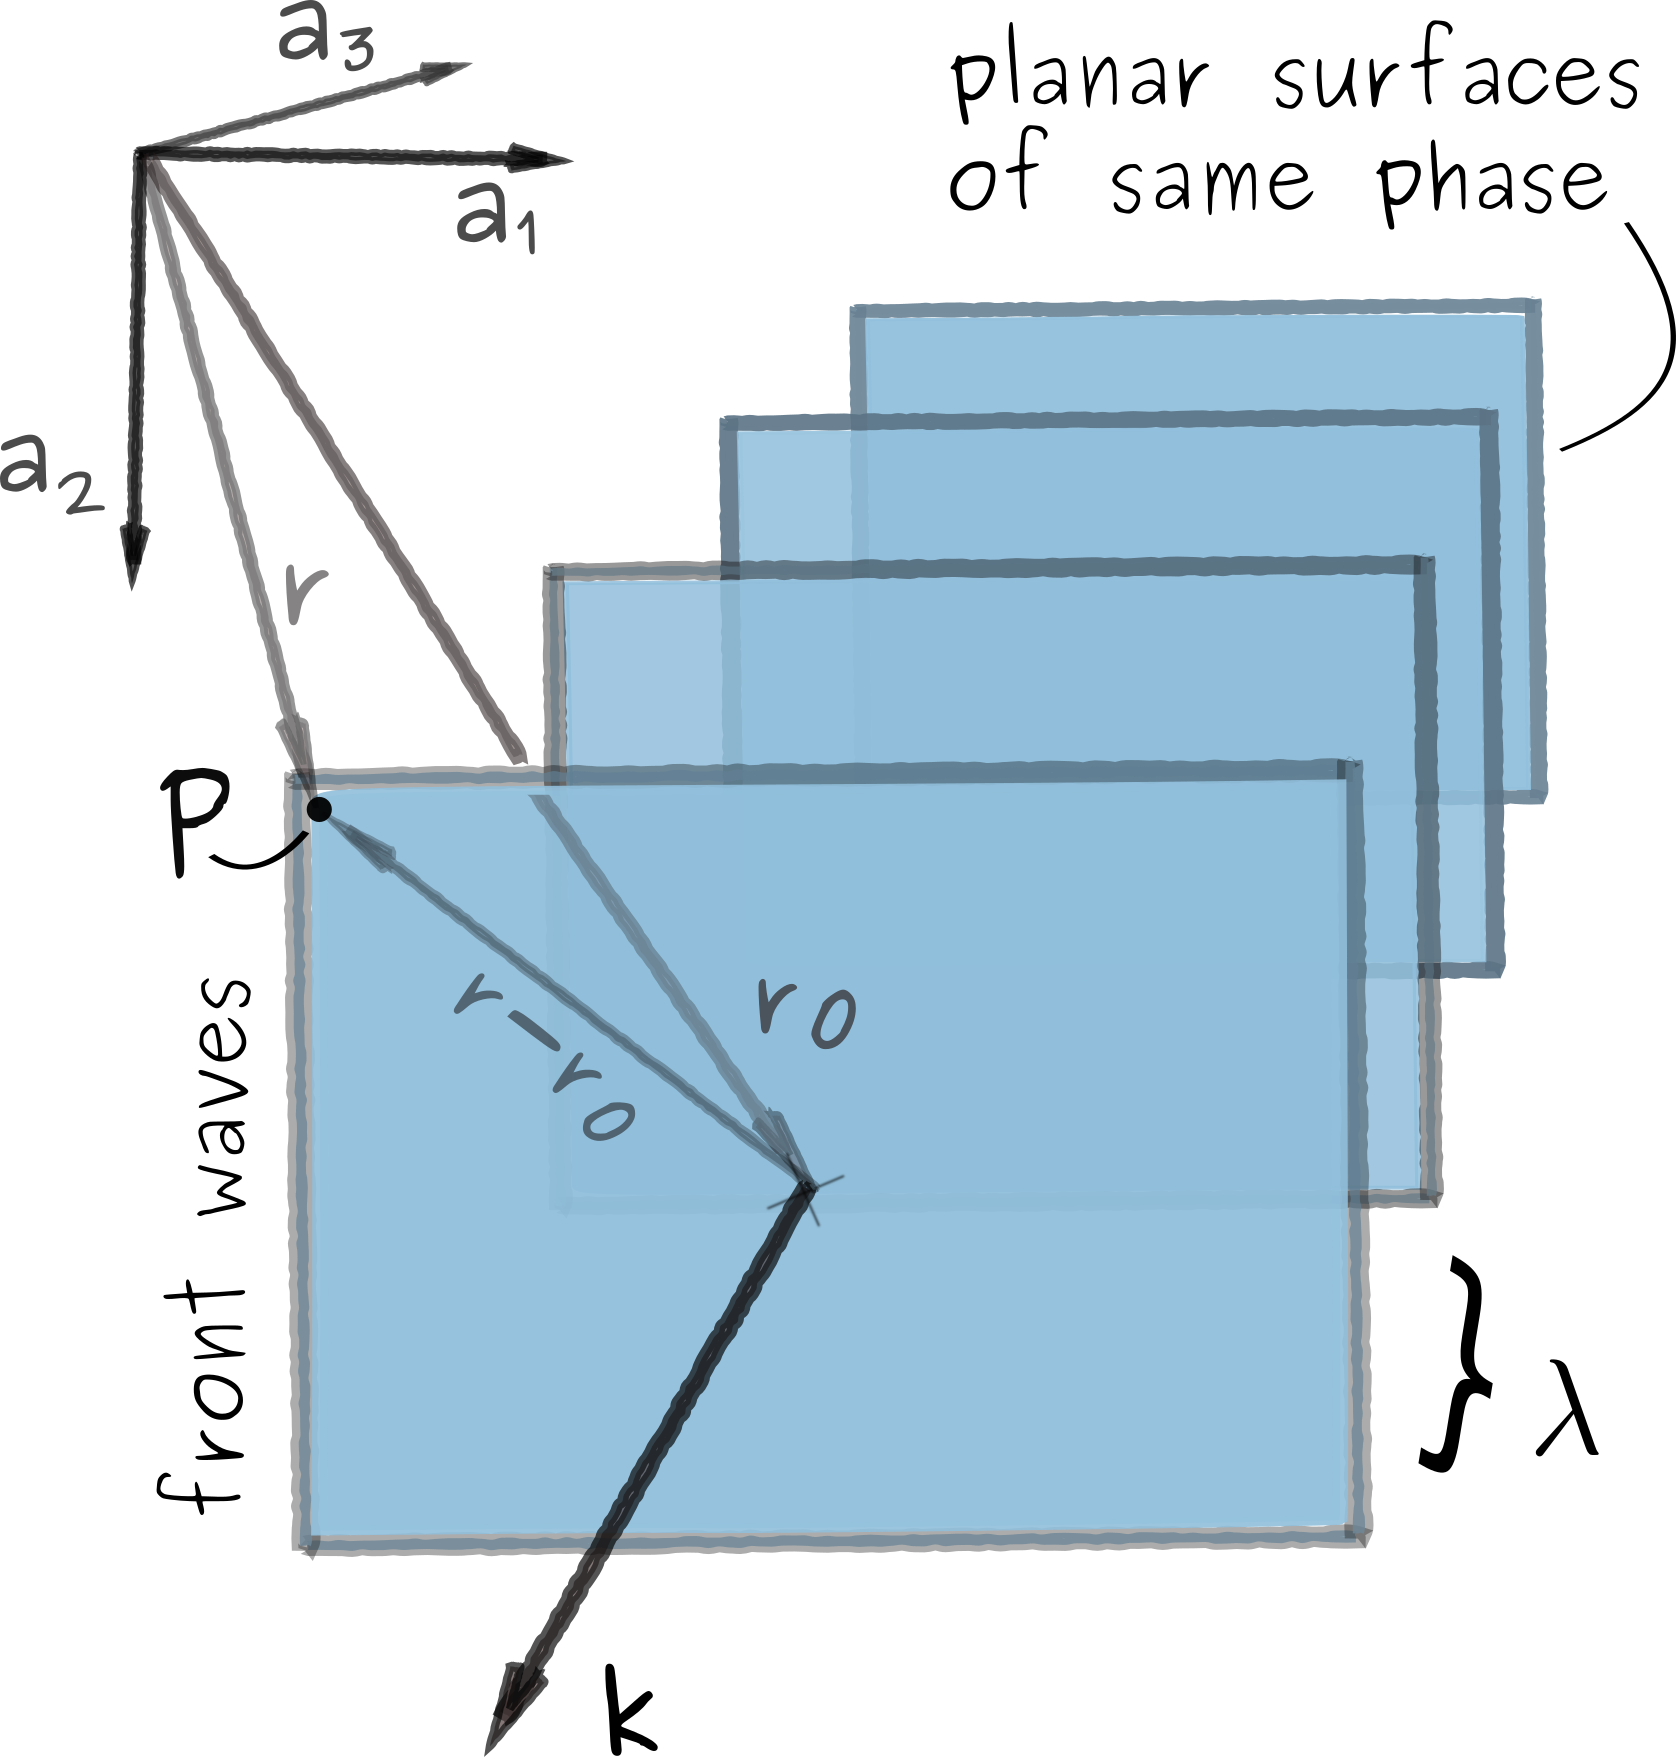
\includegraphics[width=1\linewidth]{Figures/planeWaves.png}
\captionof{figure}{Schematic drawing of plane waves and the vectors considered in this section.}
\label{Fig:planeWaves}

\end{minipage}

\vspace*{0.3cm}

We can then say that the totality of points with the same phase form an infinite plane in the real space. Another way to say this is that the particle wave will exhibit in the real space planar surfaces of same phase, oriented normal to the travelling direction $\mathbf{\hat{k}}$. Hence the name of \textit{plane waves} which we will use from now on to refer to expressions of the form:

\begin{equation}
e^{2 \pi i  \mathbf{k} \cdot \mathbf{r}}
\end{equation}






%
\subsection{Bragg's law in real space}
\label{Sec:Bragg}

\begin{minipage}{0.5\textwidth}
Consider the drawing in Fig.~\ref{Fig:Bragg}. A plane wave of wavelength $\lambda$ and wave vector $\mathbf{k}$ is incident with incidence angle $\theta$ on a set of parallel plane with Miller indices \hkl(h k l). The planes are partially transparent and partially reflective, such that the reflected beams together with the incident ones and the normal to the planes are coplanar. We ask the question: ``\textit{What is the condition that two reflected plane waves (1) and (2) will be in phase?}''. 
\end{minipage}
%---------
\begin{minipage}{0.5\textwidth}
    \centering
\captionsetup{width=.7\linewidth}
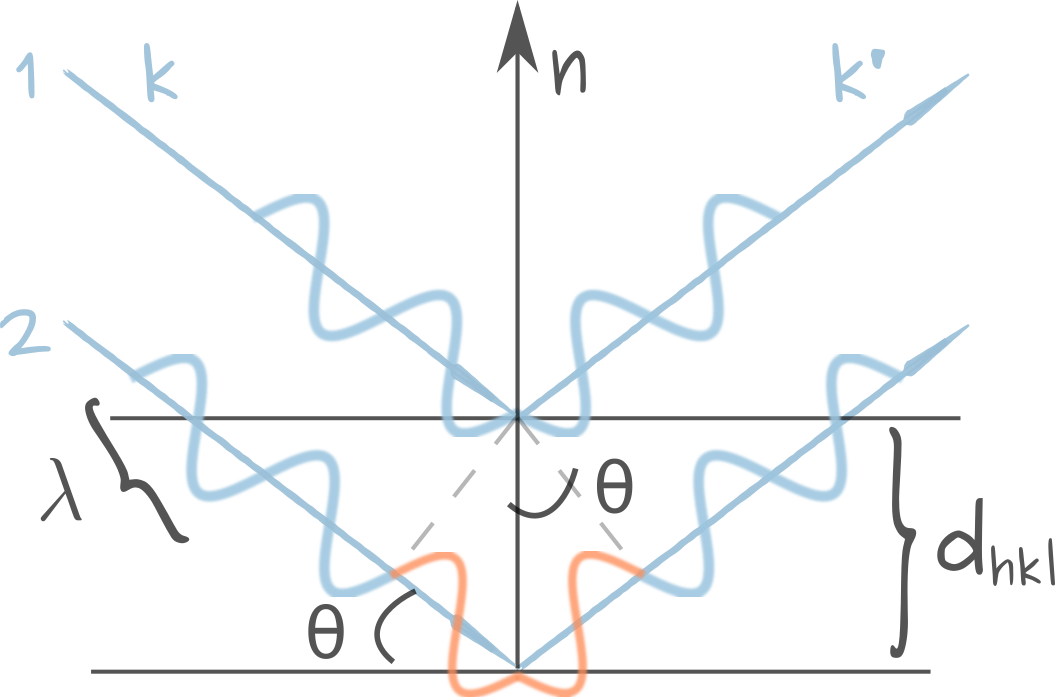
\includegraphics[width=0.8\linewidth]{Figures/Bragg.png}
\captionof{figure}{Geometrical representation of Bragg's equation in real space. The path difference of the reflected plane wave (2) with respect to (1) is shown in orange.}
\label{Fig:Bragg}
\end{minipage}

\vspace{0.5cm}
The answer is straightforward. The path difference between waves (1) and (2), shown in orange, must equal an integer number of wavelengths~\cite{Bragg13}:
$$ 2d_{hkl}\sin{\theta}=n\lambda.$$

Do note that Fig.~\ref{Fig:Bragg} is a planar section of the diffraction geometry. The diffracted beam $\mathbf{k'}$ will travel in a direction contained by a conical surface of opening angle $\pi/2-\theta$ centred around the plane normal. For every plane \hkl(hkl) in a crystal there will be a conical surface of diffracted beams, with parameters determined by the inter-planar spacing $d_{hkl}$ and the radiation wavelength $\lambda$.

In common practice we will only consider first order diffraction; instead of talking about $n$ order diffraction from planes \hkl(hkl) we will talk about first order diffraction from planes \hkl(nk nh nl). The reader will recall that the planes with Miller indices \hkl(nk nh nl) are parallel to the planes \hkl(k h l) but with an inter-planar spacing given by $d_{nh\, nk\, nl}=d_{hkl}/n$. The version of Bragg law used in diffraction is then:

\begin{equation}
2d_{hkl}\sin{\theta_B}=\lambda.
\end{equation}


The angle $\theta$ for which constructive interference occurs is known as \textit{Bragg angle}, $\theta_B$. Table~\ref{table:Bragg} shows the Bragg angles for 20 kV electrons diffracting from common wurtzite crystal planes (shown in Fig.~\ref{Fig:planeWaves}). Recall that the formula for inter-planar spacing in hexagonal unit cells is given in Eq.~\ref{eq:d_hex}.

%---------






\begin{table}[!ht]
\caption{Bragg angles for the most common planes in wurtzite materials for 20 \si{\kilo \eV} incident electrons.}
\label{table:Bragg}
\centering
\begin{tabular}{ l l c r r r}
\toprule
\tabhead{planes} & \tabhead{(hkl)} & \tabhead{$\mathbf{d_{hkl}}$} & \tabhead{$^{AlN}\theta_B$} & \tabhead{$^{GaN}\theta_B$} &  \tabhead{$^{InN}\theta_B$}\\
\midrule
  m-plane & (100)   & $\sqrt{3} a/2$   & \ang{2.74} & \ang{2.67} & \ang{2.42}\\
  c-plane & (001)   & $c$              & \ang{0.49} & \ang{0.47} & \ang{0.43}\\
  a-plane & (110)   & $a/2$            & \ang{1.58} & \ang{1.54} & \ang{1.39}\\
\bottomrule
\end{tabular}

\end{table}

Note that while the Bragg equation describes the geometric condition for diffraction, as constructive interference, to occur it does not, however, provide any information on the intensity (if any) of the diffracted beam. The real space form of this equation is only useful in determining the Bragg angles for a given wavelength and crystal structure as we have done here. More useful is the study of the direction of the diffracted beam for a given crystal structure which require the expression of some reference frame. In order to tackle this problem, it is common to express the Bragg equation to the reciprocal reference frame and introduce the Ewald sphere as we will do in the next section.


\subsection{Debye-Waller correction factor}
\label{Sec:DWf}

When we say that a crystal is a rigid structure, as we did in Section~\ref{Sec:crystalStruct} on page \pageref{Sec:crystalStruct}, we mean that over time the average positions of the atoms/molecules does not change. However, even at room temperature, the atoms exhibit thermal motion, small oscillations around their average ``real values''. While this motion does not affect the crystal structure description (\ie we can ignore small thermal effects when describing the crystal structure), it must be taken into account when the the diffraction measurement is to be interpreted.

Due to these small vibrations, the electron cloud will spread over a larger space than a frozen atom would, which will reduce the electron density, and, for our purpose, will reduce or dampen the electron-electron scattering process. An adequate approximation when accounting for atomic thermal vibration is the Debye-Waller (DW) factor $B(T)$. If we assume the scattering probability for a certain set of planes is $f_0$ when the lattice is frozen in place, \ie at \SI{0}{\kelvin}, then we can use the DW factor to correct the scattering probability $f_T$ at temperature $T$:

\begin{equation}
\label{eq:correctedScattter}
f_T=f_0 e^{-B(T)s^2}, \quad \text{with}\quad s=\frac{\sin\theta_B}{\lambda}
\end{equation}
where $s$ is half of the inverse of interplanar distance $d_{hkl}$. We will see in next chapter that $f$ is commonly known as the scattering factor and how we can calculate its value. From dimensional analysis we can see that B is proportional to the mean square displacement of the atom in the direction normal to the Bragg plane. We can also read from this equation that the intensity of the diffracted beam is reduced by a factor $e^{-B(T)s^2}$ with respect to the intensity of the same beam interacting with the sample at~$\SI{0}{\kelvin}$.

A good approximation, and the one we will use here, is to assume that for close-packed structures the atomic vibration amplitude is isotropic, such that we only require one DW parameter for each element in the crystal structure. This is not a generally valid assumption, however, first principles phonon density calculations for wurtzite-type III-V semiconductors by Schowalter \etal~\cite{Schowalter09} showed that these materials have only small anisotropies of their Debye-Waller factors.

\begin{table}[h!]
\caption{Debye-Waller fitting parameters for cubic elemental crystal from~\cite{Gao99} and the calculated DW values at 300\si{\kelvin}.}
\label{Table:DWGao}
\centering
\begin{tabular}{ l c c c c c r r}
\toprule
\tabhead{{\small Element}} & \tabhead{$a_0$} & \tabhead{$a_1$} &\tabhead{$a_2$} &\tabhead{$a_3$} & \tabhead{$a_4$} & \tabhead{{\small ME(\si{\percent})}} & \tabhead{{\small B(\si{\angstrom^2})}}   \\
\midrule
  Al & {\small 0.19} & {\small \num{0.16e-02}} & {\small \num{0.25d-05}} & {\small \num{-0.26d-08}} & {\small \num{0.10d-11}} & 1.31 &  0.83\\
  Ga & {\small 0.11} & {\small \num{0.40e-03}} & {\small \num{0.66d-05}} & {\small \num{-0.18d-07}} & {\small \num{0.19d-10}} & 0.05 & 0.49\\
  In & {\small 0.08 }& {\small \num{0.77d-02}} & {\small \num{0.48d-05}} & {\small \num{-0.12d-07}} & {\small \num{0.11d-11}} &  0.08 & 0.43\\
\bottomrule
\end{tabular}
\end{table}

Gao and Peng~\cite{Gao99} used a fourth degree polynomial regression fit to determine the temperature dependent DW factor for elemental cubic crystal from experimental data. These fit parameters are shown in Table~\ref{Table:DWGao} for the metal elements Al, Ga and In together with their estimated maximum error (ME) values. The form of the polynomial fit function is shown below:

\begin{equation*}
B(T) = a_0 + a_1T + a_2T^2 + a_3T^3 + a_4T^4
\end{equation*}

We must note here, that the measured Debye-Waller factors for defective materials will be different from that of perfect crystals since defects also scatter electrons. For this reason and the fact that first principles calculations can only be trusted if they predict experimental values, it is always  a good rule to use experimental values wherever possible. 

This being said, the literature on DW factors for nitrogen is limited and we must turn to theoretical predictions. Schowalter \etal~\cite{Schowalter09} calculated these values for a number of wurtzite structures. We show below, in Table~\ref{Table:DWSchowalter}, the values predicted for the DW factor of N in AlN, GaN and InN\footnote{ We will see later, that since N scatters electrons significantly less then the heavier metallic elements in the system, its DW factors will not carry great importance. However, we did include the computations here for completeness.}.



\begin{table}[h!]
\caption{Static correction functions for N in wurtzite materials from DFT LDA calculations~\cite{Schowalter09} at 300\si{\kelvin} and the predicted DW factor.}
\label{Table:DWSchowalter}
\centering
\begin{tabular}{ l c c  l}
\toprule
\tabhead{N in Material} &\tabhead{$\left\langle u^2_{11}(N)\right\rangle$(\si{\angstrom^2})} &\tabhead{$\left\langle u^2_{33}(N)\right\rangle$(\si{\angstrom^2})} & \tabhead{B(\si{\angstrom^2})}   \\
\midrule
  AlN & 0.0036 & 0.0034 & \num{0.28} \\
  GaN & 0.0039 & 0.0037 & \num{0.29} \\
  InN & 0.0065 & 0.0062 &\num{0.51} \\
\bottomrule
\end{tabular}
\end{table}

The Debye-Waller factor of en element, $B(el.)$, is related to the electron static correlation function, $\langle u_{\alpha}(el.) \rangle$, which is the average displacement of an atom of $el.$ in the direction $\alpha$ by:
\begin{equation*}
B(el.) = \frac{8 \pi^2}{3}\left( 2\left\langle u^2_{11}(el.)\right\rangle + \left\langle u^2_{33}(el.)\right\rangle \right).
\end{equation*}


The computations that generated the values in the tables in this section can be conveniently found in the Jupyter Notebook titled \texttt{Debye-Waller.ipynb}.




\subsection{Fourier analysis}
\label{sec:Fourier}
We have introduced the notions of crystal lattice and talked about its translational invariance under a translation vector $\vb{t}=u\vb{e_1}+v\vb{e_2}+w\vb{e_3}$ where $u,\, v,\, w$ are constants. We have also introduced the reciprocal space and that of plane waves. What is left is to tie everything together through the introduction of Fourier transform which in turn will lead us to the mathematical formulation of diffraction.

Considering the wave function description of a particle as a superposition of momentum eigenfunctions describe by vector $\vb{k}$, we now want to ask the question: \textit{``What is the relative contribution of a specific wave vector to the total function $\Psi(\vb{r})$?''}. This is a very similar question to\textit{ ``What is the contribution of the basis vector $\mathbf{e_1}$ to a given vector $\mathbf{t}=u\vb{e_1}+v\vb{e_2}+w\vb{e_3}$?''}. We know the answer to that to be $u$; easily derived from the dot product $\vb{t}\cdot \vb{e_1}$. Similarly, we can use the dot product for continuous functions of the plane wave form $\Phi = e^{2 \pi i \vb{k}\cdot \vb{r}}$ and $\Phi' = e^{2 \pi i \vb{k'}\cdot \vb{r}}$. In the bra-ket notation this is defined as:

\begin{equation*}
\braket{e^{2 \pi i \vb{k}\cdot \vb{r}}}{e^{2 \pi i \vb{k'}\cdot \vb{r}}}=\iiint e^{2 \pi i \vb{(k'-k)}\cdot \vb{r}} \dd \vb{r}=\delta(\vb{k'-k})
\end{equation*}
where the integral is over all 3D space. The delta function form underlines the fact that $\Phi$ and $\Phi'$ are orthogonal functions whenever $\vb{k'}\neq\vb{k}$ leading to the scalar product of plane wave functions to be zero.

Then, the contribution of a wave vector $\vb{k}$ to the wave function $\Psi{(\vb{r})}$ is the projection of the wave function on the momentum eigenfunction corresponding to $\vb{k}$. This also happens to be the definition of the \textit{direct Fourier transform}:

\begin{equation}
\Psi(\vb{k})=\braket{e^{2 \pi i \vb{k}\cdot \vb{r}}}{\Psi(\vb{r})}= \iiint \Psi(\vb{r}) e^{-2 \pi i \vb{k}\cdot \vb{r}} \dd \vb{r}\equiv\mathcal{F}[\Psi(\vb{r})] 
\label{eq:FT}
\end{equation}


The Fourier Transform $\mathcal{F}$ allows us to transform a wave function from the real space, $\Psi(\vb{r})$, to the momentum space, $\Psi(\vb{k})$,  by using the equation above.\footnote{ Note on the sign convention chosen: the sign of Fourier function in eq.~\ref{eq:FT} is due to the order chosen in the bra-ket and it is opposite from the crystallographic sign convention. Also note on the wave vector definition convention used here lacking the factor of $2\pi$ ($|\vb{k}|=1/\lambda$) which shows up sometimes in solid state physics. Consistent with this choice, the Fourier transform definition used here is missing the $1/2\pi$ pre-factor and reader should pay attention to the convention used when comparing with the form of these formulas with literature.} The reciprocal relationship is defined by the \textit{inverse Fourier transform}:

\begin{equation}
\Psi(\vb{r})= \mathcal{F}^{-1}[\Psi(\vb{k})] \equiv\iiint \Psi(\vb{k}) e^{\,2 \pi i \vb{k}\cdot \vb{r}} \dd \vb{k}
\label{eq:iFT}
\end{equation}


While the general analytical form of Eq.~\ref{eq:FT} does not look overly complicated, it does involve, somewhat inconveniently, a triple integral over the entire space. In the special case when the function to study is periodic, we can simplify this expression and reduce it to a discrete sum, or what is known as a \textit{Fourier series}. Any physical property of the crystal, such as charge density, carries the property of translational invariance under $\vb{t}$, which means the function for the entire crystal is periodic and can be written as an expansion of complex functions weighted by their Fourier coefficients. For instance, the direct space crystal potential can be written as the discrete inverse Fourier transform version of Eq.~\ref{eq:iFT} :

\begin{equation}
V(\vb{r}) = \sum_{\vb{k}} V_{\vb{k}} e^{\,2 \pi i \vb{k}\cdot \vb{r}},
\end{equation}
and we will show that the Fourier coefficient $V_{\vb{k}}$ are related to the diffracted wave amplitudes.

\pagebreak
%%%%%%%%%%%%%%%%%%%%%%%%%%%%%%%%%%%%%%%%%%%%%%%%%%%%%%%%%%%%%%%%%%%%%%%%%%%%%%%%
%%%%%%%%%%% Extra maths starts here
%%%%%%%%%%%%%%%%%%%%%%%%%%%%%%%%%%%%%%%%%%%%%%%%%%%%%%%%%%%%%%%%%%%%%%%%%%%%%%%%
%---------
\section{Crystallographic computations in the hexagonal system}
%----------------------
\label{chap:real+recAlg}

In the previous Section we covered the hexagonal crystal system (page \pageref{Sect:spaceLattice}) together with its basis vectors in both real (page \pageref{sec:latMB}) and reciprocal space (page \pageref{sec:recMB}). We should be ready now to tackle vectorial computations in these reference frames except for one difficulty. None of the seven crystal systems have Cartesian basis vectors and the hexagonal system is certainly not the exception. Even the cubic system is defined by non-unitary vectors. Therefore none of the usual vector identities applies.

In the following we will use the direct metric tensor to generalise the dot product for a given (non-Cartesian) crystal system both in the real and reciprocal space. We will then cover the equations for distances and angles between directions in a hexagonal system. For a good number of derivations shown here I follow the microscopy friendly textbooks~\cite{MarcTEM03} and~\cite{SoM}.

On page~\pageref{subChap:RealRec} we discuss the real to reciprocal space and inverse transformations. These are useful manipulations when it comes to combining information defined in the reciprocal space, like the diffraction condition, with information defined in real space, like position vectors in the sample. This applies, indeed, to computations of highly position-dependent diffraction information, like in the case of a polycrystalline material or defected crystal.

The alternative to using the metric tensor is to transform the parameters of interest from the crystal frame to Cartesian frame and perform the computations in the usual manner and, only after, translate the result back into the crystal frame if needed. We will use this latter approach for rotation operations which we define in the Cartesian frame on page~\pageref{subchap:basicRot}. There is another reason, besides reduction in abstraction, for wanting to move computations to a Cartesian frame or at least orthogonal frame. Regardless of the sample information we are interested in computing, the sample, the SEM geometry and the detector are all rectangular.

\subsection{The direct metric tensor}

Let us start by considering a vector $\mathbf{p}$ defined in a crystal frame with basis vectors \{$\mathbf{a_1}, \mathbf{a_2}, \mathbf{a_3}$\} by coordinates \{$p_1$, $p_2$, $p_3$\}:
\begin{equation*}
\mathbf{p}= p_1\vb{a_1} +p_2\vb{a_2}+p_3\vb{a_3}
\end{equation*}


Back to the vector $\vb{p}$ this time defined in a crystal system with basis vectors \{$\vb{a_i}, i\in (1, 2, 3)$\} and angles \{$\alpha, \beta, \gamma$\} (the list of six lattice parameters). If we are interested in finding its length we know we can use the dot product definition:%
\begin{equation*}
\vb{p}\cdot\vb{p}    =|\vb{p}|^2 \cos{(\theta=0)}
\end{equation*}
\begin{equation*}
\therefore \, |\vb{p}|  = \sqrt{\vb{p}\cdot\vb{p}}=\sqrt{p_i\vb{a_i}\cdot p_j\vb{a_j}}=\sqrt{p_i p_j \, \vb{a_i}\cdot \vb{a_j}}
\end{equation*}

If we were in a Cartesian frame \{$\vb{e}_1, \vb{e}_2, \vb{e}_3$\} we would have known that the result of the last dot product is non-zero only when $i\neq j$, \ie $\vb{a}_i\cdot \vb{a}_j=\vb{e}_i \cdot \vb{e}_j=\delta_{ij}$, and therefore $\vb{p}=\sqrt{p_1^2+p_2^2+p_3^2}$. But we are not and we don't (I didn't). Which is why we need to introduce a more general result for the dot product between two vectors.
\begin{equation*}
\vb{a_i}\cdot \vb{a_j}=|\vb{a_i}|\, |\vb{a_j}| \cos{\theta_{ij}}\equiv g_{ij},
\end{equation*}
where $\theta_{ij}$ is the usual angle between basis vectors $\vb{a_i}$ and $\vb{a_j}$ and we introduced component $ij$ of the the \textit{direct metric tensor} $\mathsf{g}$. The full $3 \times 3$ matrix form of the metric tensor can be written in terms of the six lattice parameters of a triclinic system as follows:
 \begin{equation}
 \label{eq:gmatrix}
     g = \begin{bmatrix}
    \mathbf{a_1} \cdot \mathbf{a_1}       & \mathbf{a_1} \cdot \mathbf{a_2} & \mathbf{a_1} \cdot \mathbf{a_3} \\
    \mathbf{a_2} \cdot \mathbf{a_1}       & \mathbf{a_2} \cdot \mathbf{a_2} & \mathbf{a_2} \cdot \mathbf{a_3} \\
    \mathbf{a_3} \cdot \mathbf{a_1}       & \mathbf{a_3} \cdot \mathbf{a_2} & \mathbf{a_3} \cdot \mathbf{a_3}
\end{bmatrix} =
\begin{bmatrix}
   a_1^2             & a_1 a_2 \cos{\gamma} & a_1 a_3 \cos{\beta} \\
   a_2 a_1 \cos{\gamma} & a_2^2             &a_2 a_3 \cos{\alpha} \\
   a_3 a_1 \cos{\beta}  & a_3 a_2 \cos{\alpha} &a_3^2
\end{bmatrix}.
 \end{equation}
  
For a system with higher symmetry, like the hexagonal Bravais lattice, $hP$, with lattice parameters \{$a, a, c, 90\si{\degree}, 90\si{\degree} , 120\si{\degree}\}$, the form above reduces to:
\begin{equation}
\label{eq:g3}
\mathsf{\prescript{hex}{}{g}} = \frac{a^2}{2}
\begin{bmatrix}
   2     & -1    & 0 \\
  -1     &  2    & 0 \\
   0     &  0    & c^2/2a^2
\end{bmatrix}.
\end{equation}

We are finally ready to calculate the magnitude of a vector, $\vb{p}$,  defined in a hexagonal crystal system, $\vb{p}=p_1\vb{a_1}+p_2\vb{a_2}+p_3\vb{c}$:%
\begin{equation}
\label{eq:magn3}
|\vb{p}| = \sqrt{p_i\,\, \mathsf{\prescript{hex}{}{g}_{\,ij}} \,\, p_j} = \sqrt{(a^2(p_1^2-p_1 p_2 +p_2^2) + c^2p_3^2)},
\end{equation}
the general dot product between two vectors, $\vb{p}$ and $\vb{q}$, defined in the same hexagonal crystal system, $\vb{q}=q_1\vb{a_1}+q_2\vb{a_2}+q_3\vb{c}$ :%
\begin{equation}
\vb{p} \cdot \vb{q} = p_i \,\,  \mathsf{\prescript{hex}{}{g}_{\,ij}} \, \,q_j,
\end{equation}
and the angle $\theta$ between the same two vectors:%
\begin{equation}
\label{eq:cosuvw}
\cos{\theta}=\frac{ p_i \,\,  \mathsf{\prescript{hex}{}{g}_{\,ij}} \, \,q_j}{|\vb{p}| \, |\vb{q}|}=
\frac{a^2 \left(p_1 q_1 + p_2 q_2 -\frac{1}{2}(p_1 q_2 + p_2 p_1)\right) + c^2 p_3 q_3}{|\vb{p}| \, |\vb{q}|}.
\end{equation}

It is common to ask about angles between directions rather than specific vectors. In this case it is just a matter or replacing the components $p_i$, $q_i$ with the reduced prime integers of the Miller indices of the given directions \hkl[uvw].


\textit{What about the Miller-Bravais indexing?} I hear you ask. Not to worry, we can apply an identical derivation for the four index notation hexagonal basis set \{$\vb{A_1}$, $\vb{A_2}$, $\vb{A_3}$, $\vb{C}$\}. We will denote the four-index metric tensor with $\mathsf{G}$ and follow ref.~\cite{Okamoto68} to write:
\begin{equation}
\label{eq:Ghex}
\mathsf{^{hex}G}=\begin{bmatrix}
    \mathbf{A_1} \cdot \mathbf{A_1}       & \mathbf{A_1} \cdot \mathbf{A_2} & \mathbf{A_1} \cdot \mathbf{A_3} & \mathbf{A_1} \cdot \mathbf{C} \\
    \mathbf{A_2} \cdot \mathbf{A_1}       & \mathbf{A_2} \cdot \mathbf{A_2} & \mathbf{A_2} \cdot \mathbf{A_3} & \mathbf{A_2} \cdot \mathbf{C} \\
     \mathbf{A_3} \cdot \mathbf{A_1}       & \mathbf{A_3} \cdot \mathbf{A_2} & \mathbf{A_3} \cdot \mathbf{A_3} & \mathbf{A_3} \cdot \mathbf{C} \\
    \mathbf{C} \cdot \mathbf{A_1}       & \mathbf{C} \cdot \mathbf{A_2} & \mathbf{C} \cdot \mathbf{A_3} & \mathbf{C} \cdot \mathbf{C}
\end{bmatrix} =\frac{a^2}{2}\begin{bmatrix}
2 & -1 & -1 & 0 \\
-1 & 2 & -1 & 0 \\
-1 & -1 & 2 & 0 \\
0 & 0 & 0 & 2c^2/a^2 
\end{bmatrix}
\end{equation}

The magnitude of the same vector $\vb{p}$ this time  with components \{$P_1$, $P_2$, $P'$, $P_3$\} corresponding to the four-vector basis, $\vb{p}=P_1 \vb{A}_1 + P_2\vb{A}_2 +P'\vb{A}_3 +{P_3}\vb{C}$ is:
\begin{equation}
\label{eq:pmag}
|\vb{p}| = \sqrt{P_i\,\, \mathsf{\prescript{hex}{}{G}_{\,ij}} \,\, P_j} = \sqrt{(3a^2(P_1^2+P_1 P_2 +P_2^2) + c^2P_3^2)},
\end{equation}
which is similar but not the same as Eq.~\ref{eq:magn3}, note the sign difference. For the same vector the coordinates in four-vector basis are going to be smaller than the coordinates in the three-vector basis, since there are more vectors to contribute. A word of advice for the reader, don't be tempted to apply the vector length derivation to the Miller and Miller-Bravais notation of directions, remember the discussion on page~\pageref{disc:millervector}. 

The angle between two vectors, $\vb{p}=P_i \vb{A}_i$ and $\vb{q}=Q_i \vb{A}_i$, defined using the four-vector basis of a hexagonal lattice is then, similarly to Eq.~\ref{eq:cosuvw}:
\begin{equation}
\cos{\theta}=\frac{ P_i \,\,  \mathsf{\prescript{hex}{}{G}_{\,ij}} \, \,G_j}{|\vb{p}| \, |\vb{q}|}=
\frac{a^2 \left(3(P_1 Q_1 + P_2 Q_2) + \frac{3}{2} (P_1 Q_2 + P_2 P_1)\right) + C^2 P_3 Q_3}{|\vb{p}| \, |\vb{q}|}.
\end{equation}


\subsection{The reciprocal metric tensor}

On page \pageref{sec:recHex} we covered, to some extent, the reciprocal hexagonal lattice and its basis vectors in both the linearly independent form of \{$\vb{a^*_1}$, $\vb{a^*_2}$, $\vb{c^*}$\} and the linearly dependent \{$\vb{A^*_1}$, $\vb{A^*_2}$, $\vb{A^*_3}$, $\vb{c^*}$\}. 

The \textit{reciprocal metric tensor}, can be derived in much the same way as the real space one, by doing the dot product between all the pairs of basis vectors: $\mathsf{g_{ij}^*}=\vb{a_i^*}\cdot\vb{a_j^*}$. It is also, quite conveniently, the inverse of the real space metric tensor: $\mathsf{g_{ij}^*}=\mathsf{(g_{ij})}^{-1}$, such that for the reciprocal hexagonal lattice with parameters \{$a^*$, $\,a^*$,\, $\,c^*$, 90\si{\degree}, 90\si{\degree}, 60\si{\degree}\} can easily be written out to be:
\begin{equation}
\label{eq:gstar}
     \mathsf{^{hex}g^*}  =  \begin{bmatrix}
    \mathbf{a_1^*} \cdot \mathbf{a_1^*}       & \mathbf{a_1^*} \cdot \mathbf{a_2^*} & \mathbf{a_1^*} \cdot \mathbf{c^*} \\
    \mathbf{a_2^*} \cdot \mathbf{a_1^*}       & \mathbf{a_2^*} \cdot \mathbf{a_2^*} & \mathbf{a_2^*} \cdot \mathbf{c^*} \\
    \mathbf{c^*} \cdot \mathbf{a_1^*}       & \mathbf{c^*} \cdot \mathbf{a_2^*} & \mathbf{c^*} \cdot \mathbf{c^*}
\end{bmatrix}= \mathsf{(^{hex}g)}^{-1} =
    \frac{2}{3a^2}\begin{bmatrix}
   2       & 1           & 0 \\[6pt]
   1       & 2           & 0 \\[6pt]
   0       & 0           & 3a^2/2c^2
\end{bmatrix} 
\end{equation}
The lattice parameters are inverted with respect to the real metric tensor given in Eq.~\ref{eq:g3}, as expected, and we also gained a normalisation factor of $1/3$ from the determinant. But more notably, the form of the matrix is different to all the other hexagonal metric tensors. The minus signs present in 1) Eq.~\ref{eq:g3}, 2) Eq.~\ref{eq:Ghex} and, as we will see, in 3) Eq.~\ref{eq:Gstar} are missing here. This observation is consistent with the comments made for Fig.~\ref{Fig:recBasis} on page~\pageref{Fig:recBasis}, namely that the hexagonal reciprocal space lattice defined by three basis vectors is different 1) the real space  hexagonal lattice defined with three basis vectors 2) the one defined with four basis vectors and 3) the reciprocal hexagonal lattice defined with four basis vectors. Just to reiterate, interchanging between basis sets needs a bit of thought.

We can write out, similarly to equation~\ref{eq:magn3}, the length of a generic reciprocal space vector $\vb{g}=g_1\vb{a_1^*}+g_2\vb{a_2^*}+g_3\vb{a_2^*}$ (written conveniently for Einstein summation) from the dot product with itself:
\begin{equation}
\label{eq:gdot}
|\vb{g}| = \sqrt{g_i \, \mathsf{g_{ij}^*}\, g_j}
\end{equation}

In terms of the four index notation, the reciprocal metric tensor $\mathsf{G^*}$ is:
\begin{equation}
\label{eq:Gstar}
\mathsf{^{hex}G^*} =\frac{2}{9a^2}\begin{bmatrix}
2 & -1 & -1 & 0 \\
-1 & 2 & -1 & 0 \\
-1 & -1 & 2 & 0 \\
0 & 0 & 0 & 9a^2/2c^2 
\end{bmatrix}
\end{equation}
Which looks very similar to the real space four-index notation metric tensor $\mathsf{^{hex}G}$ in Eq.~\ref{eq:Ghex} with inverse lattice parameters; as expected, since the real and reciprocal four-basis vectors are parallel to one other.



\subsection{The interplanar spacing}

We now have all the tools to calculate the length of the translation vector in the hexagonal system reciprocal lattice, $\vb{g}_{hkl}=h\vb{a_1^*}+k\vb{a_2^*}+l\vb{c^*}$ defined in Eq.~\ref{eq:ghkl}. The identity in Eq.~\ref{eq:gdot} reduces to: 
\begin{equation*}
|\vb{g}_{hkl}|= \sqrt{\frac{4}{3a^2}(h^2 + k^2 + h k) + \frac{1}{c^2}l^2)}
\end{equation*}


Such that we could, finally, derive the expression for the distance between a set of planes \hkl{hkl} in a hexagonal system defined in Eq.~\ref{eq:dhkl}:
\begin{equation}
^{hex}d_{hkl} = \frac{1}{\sqrt{\frac{4}{3a^2} (h^2 + k^2 + h k) + \frac{1}{c^2}l^2}}
\label{eq:d_hex}
\end{equation}
We can also find the distance between a set of hexagonal system planes \hkl{hkil} given in Miller-Bravais notation:

\begin{equation}
^{hex}d_{hkil} = \frac{1}{\sqrt{\frac{4}{3a^2} (h^2 + k^2 + i^2 + h k + k i + i h) + \frac{1}{c^2}l^2}}
\label{eq:d_hex_MB}
\end{equation}

Table~\ref{Table:dhkl} shows a few examples of calculated interplanar distances for common families of planes in wurtzite nitride systems (see Fig.~\ref{Fig:planes}). Spot that the distance between consecutive \textit{c-planes} is the lattice parameter \textit{c} while the one between \textit{a-planes} is half the lattice parameter \textit{a}. 


\begin{table}[h!]
\caption{Calculated interplanar distances in wurtzite nitrides.}
\label{Table:dhkl}
\vspace{-0.5cm}
\centering
\begin{longtable}{lcccc}\toprule
             & \multicolumn{4}{c}{\tabhead{Interplanar spacing for set of planes \hkl{hkl} [\si{\angstrom}]}}\\ \cmidrule{2-5}
\tabhead{System (a[\si{\angstrom}], c[\si{\angstrom}])}        &  a-plane \hkl{110} & r-plane \hkl{1-12} & m-plane \hkl{100} & c-plane \hkl{001} \\ \midrule
AlN (3.11, 4.98) &   1.56 & 1.83 & 2.69 &  4.98\\
GaN (3.19, 5.19)  &  1.60 & 1.89 & 2.76 & 5.19  \\
InN (3.53, 5.70) &   1.77 & 2.08 & 3.07 & 5.70 \\
\bottomrule
\end{longtable}
\end{table}




\subsection{To the reciprocal space and back}
\label{subChap:RealRec}


While the equivalence between reciprocal vector absolute value and inverse of the distance between planes is clear, other transformations between the two vector spaces require a bit more work. Let us start with a vector $\vb{p}$ with components \{$p_i$, $i \in (1, 2, 3)$\} in the real space, $\vb{p}=p_i \vb{a_i}$. This vector must exist independent of the reference frame, so let us give it components \{$p_i^*$, $i \in (1, 2, 3)$\} in the reciprocal space: $\vb{p}=p^*_i\vb{a}^*_i$ such that:
\begin{equation}
\label{eq:pvect}
\vb{p}=p_i \vb{a}_i=p^*_i\vb{a}^*_i.
\end{equation}

If, in the latter equality, we dot product both sides by $\vb{a}_j$ and use both the property of the reciprocal lattice, given in Eq.~\ref{eq:adotastar},  and the definition of the direct metric tensor, $\mathsf{g_{ij}}=\vb{a}_i\cdot\vb{a}_j$ then we find that:
\begin{equation}
\label{eq:directg}
p^*_j=p_i \mathsf{g_{ij}}
\end{equation}
Which tells us how to find the components of the vector in the reciprocal space. 

Alternatively, if we know the components of the vector in reciprocal space and want to define it in the real space, we dot product the right side of the last equality in Eq.~\ref{eq:pvect} by $\vb{a}^*_j$, and use the definition of the reciprocal metric tensor this time, $\mathsf{g^*_{ij}}=\vb{a}^*_i\cdot\vb{a}^*_j$, to find:
\begin{equation}
\label{eq:pi}
p_j=p_i^* \mathsf{g^*_{ij}}
\end{equation}

Similarly, if are interested in finding the reciprocal basis vectors, $\vb{a}^*_i$, knowing the real space basis vectors $\vb{a}_i$, we replace $p_i$ with the identity in Eq.~\ref{eq:pi} to find:
\begin{equation}
\label{eq:astar}
\vb{a}^*_i=\mathsf{g^*_{ij}} \mathbf{a}_j,
\end{equation}
and, inversely, 
\begin{equation}
\label{eq:directga}
\vb{a}_i=\mathsf{g_{ij}} \mathbf{a}^*_j.
\end{equation}

Notice the difference in position of the metric tensor in equations \ref{eq:directg} and \ref{eq:directga}. Another way to remember this is that the rows of the metric tensor are the components of the direct basis vector in terms of the reciprocal basis vectors, as explained in \textit{Introduction to CTEM} pg. 17 ~\cite{MarcTEM03}, and the columns of the metric tensor contain the reciprocal components of a vector in therms of the real space components. 


\subsubsection{The reciprocal lattice basis vectors}
\label{sec:crossProd}

On page~\pageref{eq:3recvectors} I made a promise to show where the form for the hexagonal reciprocal basis vectors (Eq.~\ref{eq:3recvectors}) comes from.
Let us finally apply the reciprocal space vector definition in Eq.~\ref{eq:recVectors} to the hexagonal lattice. If we now make an attempt at writing out the cross products between two basis vectors of a crystal lattice, $\mathbf{a_p}$ and $\mathbf{a_q}$\footnote{ The index notation is going to be a bit crazy in this section; we are trying to annotate both different basis vectors and components of said vectors. The Einstein summation rules discussed on page~\pageref{par:Einstein} continue to apply.}:
\begin{equation*}
\vb{a_p} \times \vb{a_q} = \Omega \,\, \epsilon_{ijk} \, \vb{a_p}_{,i}\,  \vb{a_q}_{,j} \,   \vb{a^*}_k
\end{equation*} 
where $\Omega$ is the volume of the unit cell. We have used a new symbol, $\epsilon_{ijk}$, known as the \textit{normalised permutation symbol} which can take three values depending on the order of indices $\{h, k, l\}$: 
\begin{equation*}
\epsilon_{ijk}=
    \begin{cases}
      +1, & \text{if}\ {i,j,k} \text{ are an even permutation of 123}, \\
      -1, & \text{if}\ {i,j,k} \text{ are an odd permutation of 123},\\
      0, & \text{otherwise} .
    \end{cases}
\end{equation*}

$\vb{a_p}_{,i}$ is the component $i$ of the basis vector $\vb{a_p}$ and surely can only take the value 1 when $p=i$, \ie $\vb{a_p}_{,i}=\delta_{pi}$. In the same manner,  $\vb{a_q}_{,j}=\delta_{qj}$.

Since the cross product of two basis vectors points in a direction normal to both vectors, and since in a non-Cartesian system this will not necessary coincide with the direction of the third basis vector, we had to use a different trick. Namely, the definition of the reciprocal basis vectors (Eq.~\ref{eq:recVectors}) which is the reason why we ended up with a reciprocal vector component in the equation above in the first place anyway. Nevertheless, the equation above does not lead us very far in the attempt to write out the reciprocal basis vectors in terms of the real space one. We can however fix that by converting the components of this vector to the real space using Eq.~\ref{eq:astar} derived above. 

Finally, we can write: 

\begin{equation*}
\vb{a_p} \times \vb{a_q} = \Omega \,\, \epsilon_{pqk}\, \,  g^*_{km} \vb{a_m}.
\end{equation*}

For the hexagonal lattice basis set we just replace the reciprocal metric tensor with the form given in Eq.~\ref{eq:gstar}. This would lead us end up with the reciprocal lattice vectors in on page~\pageref{eq:3recvectors}.

\subsection{Rotations in Cartesian frame}
\label{subchap:basicRot}
It is common in crystallographic calculations to want to express a tensor parameter known in one reference in a different reference frame; assuming we can figure out the position of the new reference frame in the old reference frame. For instance, mapping the electron beam scan in the sample frame (a task made especially challenging by the high sample tilt used in electron diffraction techniques, which the SEM is not very well designed to account for ~\cite{Nolze07}), involves moving electron scan positions between the beam frame and the sample frame. Assuming the scanning directions $x$ and $y$ are truly perpendicular, that the $x$ scanning direction is indeed parallel to the tilt axis of the sample and that the magnification and spot size are not significantly affected by the tilt (\ie parallel beam at high magnification) then the relationship between the basis vectors of two frames is a simple rotation. A similar transformation must be done for translating the escaping electron beam positions from the sample frame to the detector frame~\cite{Britton16}. 

Unfortunately, simply calling an action rotation, suffers from many ambiguities. In crystallography, when we talk about rotation we refer to a very well defined transformation. In a right handed system\footnote{ $(x, y, z)$ follow the thumb, index and middle fingers of the right hand} -- first source of ambiguity --, a rotation of the coordinate system (CS) around a given axis is the clockwise rotation in the plane normal to that axis as the viewer looks in the direction pointed by the axis. Another way of describing the clockwise rotation is the right hand rule, \ie holding the thumb in the direction of the chosen axis of rotation, the rest of the fingers point in the direction of rotation. 

If you just looked at your right hand fingers going, in fact, anti-clockwise then you'll understand why I call rotations confusing. It matters where the rotations axis, or finger is pointing -- second source of confusion. You do need to align your viewing direction with the direction of the rotation axis, that is you need to awkwardly turn your right hand such that the thumb points to were you are looking. Voil\`{a}, clockwise rotation. Also, my activity for months during my PhD. 

Another possible ambiguity is whether we refer to a \textit{active} or a \textit{passive} rotation:
\begin{itemize}
\item A passive, or alias transformation, like the one above, acts on the coordinate system. It rotates the CS clockwise around a given axis while keeping the position of the object of interest fixed.
\item An active, or alibi transformation acts on the object. More explicitly, the active rotation affects the position vector of the object whose coordinates are described in a fixed CS. The direction of rotation is opposite to the passive one and therefore anticlockwise.
\end{itemize}
It should be obvious that a passive rotation of an object by an angle $\theta$ around a given axis is equivalent with a passive rotation of its coordinate frame by an angle $-\theta$ around the same axis.

The mathematical form of these transformations in 3D can be written as $3\times 3$ matrices, $\mathcal{R}$. In the case in which the axis of rotation is one of the basis vectors we call the transformation a basic rotation. The tree basic rotation matrices for a right handed Cartesian frame are given in Appendix~\ref{Chap:rotations}. 

Yet another source of ambiguity is the manner in which we apply the rotation matrix. Through this work we pre-multiply the rotation matrix with the position column vector: $\mathbf{v'}=\mathcal{R}(\theta)\mathbf{v}$. This leads us to the unambiguous definition of rotation we will use: \textit{The anticlockwise rotation of a position vector in column form, $\mathbf{v}$, given in a right handed CS, around the rotation axis $\mathbf{n}$ leads to a new position which can be calculated by pre-multiplying the rotation matrix $\mathcal{R_{\mathbf{n}}}$ by the position vector: $\mathcal{R_{\mathbf{n}}} \mathbf{v}$ }. For any property in this definition changed the rotation direction flips. For instance, post-multiplying the rotation matrix with row vector leads to a clockwise rotation. 

A useful property of the rotation matrix is that the inverse of a rotation can be calculated by simply transposing the matrix ($\mathcal{R} \mathcal{R}^\intercal  = \mathcal{I}$). Another property is that the product of rotation matrices is yet another rotation matrix. Even in the case in which the rotation axis is not just a basis vector, the rotation can be broken down in maximum tree basic rotations. 

This latter scenario describes another rotation formalism known as \textit{Euler rotation} in terms of Euler angles; the rotation is given as a set of three angles which describe three successive rotations around a combination of the axes \hkl{\mathbf{x}, \mathbf{y}, \mathbf{z}}. Since matrix multiplication is not commutative, the order of the chosen axis is important and a lack of knowledge of the chosen convention makes the Euler notation ambiguous, in a yet different way. EBSD orientation mapping uses, for instance, the Bunge convention~\cite{Bunge}, which orders the Euler angles as: $(\phi_1, \phi_2, \phi_3)$ around $(\mathbf{x}, \mathbf{z}, \mathbf{x})$, such that the total rotation is given by:
\begin{equation*}
^{Bunge}\mathcal{R}_{Euler}(\phi_1, \phi_2, \phi_3) = \mathcal{R}_x(\phi_3) \mathcal{R}_z(\phi_2) \mathcal{R}_x(\phi_1).
\end{equation*}
This series of rotations for a coordinate system from one position to another can be read as a rotation of $\phi_1$ around the basis vector $\mathbf{x}$ followed by  $\phi_2$ around  $\mathbf{z}$ and, finally, $\phi_3$ around $\mathbf{x}$. 

There are application for which neither the rotation matrix nor the Euler angle formalism are fully adequate, not least due to the ambiguities that need to be ironed out. One alternative is the \textit{quaternion representation}. Quaternions are four-dimensional vectors, or can be seen as complex numbers with two extra non-real parts of the from $\hat{\mathbf{q}}=q_i \mathbf{i} + q_j \mathbf{j} +q_k \mathbf{k} +q_r= \begin{bmatrix}q_i, q_j, q_k, q_r \end{bmatrix}$. A quaternion of this form describes a rotation around a rotation axis $\mathbf{n} = \begin{bmatrix} n_x, n_y, n_z\end{bmatrix}$ by an angle $\theta$ such that $q_i=n_x \sin{(\theta/2)}$, $q_j=n_y \sin{(\theta/2)}$, $q_j=n_z \sin{(\theta/2)}$ and $q_r= \cos{(\theta/2)}$. Quaternion maths will be faster on a computer compared to rotation matrices since the trigonometric functions are absent and it requires fewer operations per transformation. 

Rowenhost \etal~\cite{Rowenhorst15} worked out the complete conversions between the rotation formalisms used in material science (including the Rodrigue-Frank vectors and homochronic vectors) and provided extensive open source Fortran-90 libraries with the implementations. The GitHub repository of Prof. De Graef~\cite{3Drot} contains Fortran95, IDL, MatLab, and C++ implementations for the rotations and conversions as well.


Now that we covered how to do rotations in a Cartesian frame we will go over transformations to and from the crystal frame.


\subsection{Crystal to Cartesian frame and the structure matrix}

While computations in the crystal frame conserves the symmetry of the crystal and keeps the equations somewhat intuitive, there are undeniable benefits to bringing the calculations into the Cartesian frame as well. If only because implementing non Cartesian vectorial manipulation requires extra work, but ultimately because we want to project the information on a square detector or screen. We are interested in writing out the path of transforming from both the real and reciprocal hexagonal space to the Cartesian system. 

The easiest and most common way of defining a Cartesian frame with basis vectors $\mathbf{e}_i$ with respect to the crystal frame with basis vectors $\mathbf{a}_i$ and corresponding reciprocal space vectors  $\mathbf{a}^*_i$ is as follows:
\begin{itemize}
\item  $\mathbf{e}_1$ is the unit vector parallel to $\mathbf{a}_1$:
\begin{equation}
\label{eq:e1}
\mathbf{e}_1 =\frac{\mathbf{a}_1 }{|\mathbf{a}_1| } 
\end{equation}

\item  $\mathbf{e}_3$ is the unit vector parallel to $\mathbf{a}^*_3$: 
\begin{equation}
\mathbf{e}_3 =\frac{\mathbf{a}^*_3 }{|\mathbf{a}^*_3| } 
\end{equation}

\item and $\mathbf{e}_2$ completes the right handed Cartesian reference frame:
\begin{equation}
\label{eq:e3}
\mathbf{e}_2 = \mathbf{e}_3 \times \mathbf{e}_1 .
\end{equation}
\end{itemize}

Let us consider a vector $\mathbf{p}= p_i \vb{a}_i$, whose components in the Cartesian frame are~$x^p_i$. Since $\mathbf{p}= p_i \vb{a}_i=x^p_i\vb{e}_i$ it means that we could find a coordinate transformation matrix $\mathsf{a_{ij}}$ which relates the components $p_i$ and $x^p_i$: 
\begin{equation}
\label{eq:aij}
x^p_i = \mathsf{a_{ij}}  p_i
\end{equation}

The components of the matrix $\mathsf{a_{ij}}$ can be found by rewriting the lengths of the lattice vectors in Eq.'s~\ref{eq:e1} to~\ref{eq:e3} in terms of the direct and reciprocal matrix tensors. For instance, $|\vb{a_1}|=\sqrt{\mathsf{g_{11}}}$ (see Eq.~\ref{eq:gmatrix}). For the rest of the beautiful derivation we send the reader to page 140 of ref.~\cite{SoM}. The final matrix will have elements containing both the direct and reciprocal metric tensor. We give here the form of matrix $\mathsf{a_{ij}}$, also known as the \textit{direct structure matrix}, for a hexagonal lattice:
\begin{equation}
\mathsf{^{hex}a_{ij}}=\begin{bmatrix}
a & \frac{-a}{2}         & 0 \\[0.3em]
0 & \frac{\sqrt{3} a}{2}  & 0 \\[0.3em]
0  &   0          & c 
\end{bmatrix}
\end{equation}

If we want to translate a reciprocal space vector to the same Cartesian frame, we have to introduce a second matrix $\mathsf{b_{ij}}$ known as the \textit{reciprocal structure matrix}. We start now with a vector $\vb{g}$ with components $g_i$ in the reciprocal space: $\vb{g}=g_i \vb{a}^*_i$. The same vector will have components $x^g_i$ in the Cartesian frame: $\vb{g}=x^g_i \vb{e}_i = g_i \vb{a}^*_i$ such that $x^g_i=\mathsf{b_{ij}} g_i$. We can use the reciprocal structure matrix $\mathsf{g^*_{ij}}$ (Eq.~\ref{eq:astar}) to rewrite the reciprocal basis vectors $\vb{a}^*_i$ in terms of the real ones $\vb{a}_j$ such that: 
\begin{equation*}
\vb{g}=x^g_i \vb{e}_i = g_i \,\mathsf{g^*_{ij}} \, \vb{a}_j,  
\end{equation*}
where we can now use the direct structure matrix $\mathsf{a_{ij}}$ (Eq.~\ref{eq:aij}) to relate the quantities $x^g_i$ and $g_l \,\mathsf{g^*_{lj}}$:
\begin{equation*}
x^g_i = \mathsf{a_{ij}} \, g_l \,\mathsf{g^*_{lj}} = \mathsf{a_{ij}} \, \mathsf{g^*_{jl}} \,  g_l. 
\end{equation*}

We can now define the reciprocal structure matrix for a hexagonal lattice, $\mathsf{^{hex}b_{ij}}$:
\begin{equation}
\mathsf{^{hex}b_{ij}} = \mathsf{^{hex}a_{ij}} \, \mathsf{^{hex}g^*_{jl}} = \begin{bmatrix}
\frac{1}{3a} & 0 & 0 \\[0.3em]
\frac{\sqrt{3}}{3a} & \frac{2\sqrt{3}}{3a} & 0 \\[0.3em]
0 & 0 & \frac{1}{c}
\end{bmatrix}.
\end{equation}


\subsection{Metric tensor implementations}
I took the time to write out a good number of equations in this section. While these are well established and, probably, well  understood vectorial manipulation in the world of X-ray diffraction, electron microscopists don't often incorporate basis transformations language in their work. I make this claim based on the observation that, while the implementation would be trivial, there is a lack of mature, accessible and easy to plug-and-play (ideally open) software out there to answer some of the crystallographic questions the material scientists might ask when using an SEM as a characterisation tool. 

Until a \textit{Python} library is available and documented for crystallographic basis set computations, I leave the reader with a \href{http://ssd.phys.strath.ac.uk/resources/crystallography/crystallographic-direction-calculator/}{web tool}\footnote{ Link address is: \href{http://ssd.phys.strath.ac.uk/resources/crystallography/crystallographic-direction-calculator/}{http://ssd.phys.strath.ac.uk/resources/crystallography/crystallographic-direction-calculator/} .}, albeit limited in capabilities, written by Albes Koxhaj, an excellent summer project student in the SSD department who implemented a few of the equations here, and revised by me. The last two blocks of calculators in this tool were written to find the coordinates, in the crystal frame, of the normal direction on a given plane \hkl(hkl) or \hkl(hkil). For a hexagonal plane, we show that there are two special conditions in which the normal to a plane can be reduced to Miller indices \hkl[uvw]. The first case is when the $\mathbf{c}$-direction is parallel to the plane ($l=0$) such that the lattice parameters can be removed from the indices and we are left with integer numbers. The second case is when the $\mathbf{c}$-direction is normal to the plane ($h=l=0$ or $h=l=i=0$), when the normal is along $\mathbf{c}$ in both the real and reciprocal space. Any other case will keep coordinates dependent on the lattice parameters $a, c$ which would make them unlikely to be reduced to integers. 

I also wrote a few Python lines in the Jupyter notebook \texttt{grainNormal.ipyb}, showing the steps needed to calculate the surface normal in the crystal frame of individual grains from the Euler angles of an EBSD map by applying the identities in this section. 
 
\emph{EMsoft}~\cite{EMsoftpaper} contains Fortran90 implementations of the metric tensor tensor formalism. The source code can be found in the \texttt{crystal.f90} and \texttt{symmetry.f90} modules in Source/EMsoftLib path on the GitHub page~\cite{EMsoft}.

\pagebreak

\section{Wurtzite symmetry}
\label{sec:Wsymmetry}
I wrote a somewhat comprehensive introduction to symmetry in the wurtzite system in Appendix~\ref{Chap:Symmetry}. This is aimed at a complete novice to crystallography which I was at the beginning of this journey. I tried to keep it textbook level by following the Symmetry chapter in \textit{Structure of Material: An Introduction to Crystallography, Diffraction and Symmetry}~\cite{SoM} and focusing on the symmetry operations relevant for this crystal system. Though it can look daunting and dry, I was told, I would recommend the reader to adventure a look though it if they want want to understand were the symmetry information in this section comes from. I believe it makes for a decent read and I added a lot of helping figures and beautiful  \href{https://sourceforge.net/projects/rayshade/}{Rayshade}\footnote{ Link is \href{https://sourceforge.net/projects/rayshade/}{https://sourceforge.net/projects/rayshade/}.} 3D renderings. I wrote my own input files for these renderings based on the input  \href{http://som.web.cmu.edu/frames2.html}{\emph{*.ray} files}\footnote{ Link is \href{http://som.web.cmu.edu/frames2.html.}{http://som.web.cmu.edu/frames2.html}.} developed by Marc De Graef~\cite{DeGraef98} with the purpose of teaching the crystallography group symmetry~\cite{teachingPointGroup}. My scripts can be found at this \href{https://github.com/elena-pascal/SEM-diffraction/tree/master/Wurtzite_symmetry/}{GitHub repository}\footnote{ Link is \href{https://github.com/elena-pascal/SEM-diffraction/tree/master/Wurtzite_symmetry}{https://github.com/elena-pascal/SEM-diffraction/tree/master/Wurtzite\_symmetry}.}. 

On page~\pageref{chap:int} of the same Appendix, I also went over how to decipher the symbols in the \textit{ International Tables for Crystallography, Volume A}~\cite{IntTableCrysA}, a skill indispensable to any crystallographer. Specifically, pages 584-858 of the \textit{Tables}, covering space group $\mathbf{P6_3mc}$, are explained in detail.

In the following section I will assume the reader has working knowledge of crystallographic language. You have been warned!


\subsection{The \texorpdfstring{$\mathbf{P6_3mc}$}{P63mc} space group }

\begin{figure}
    \centering
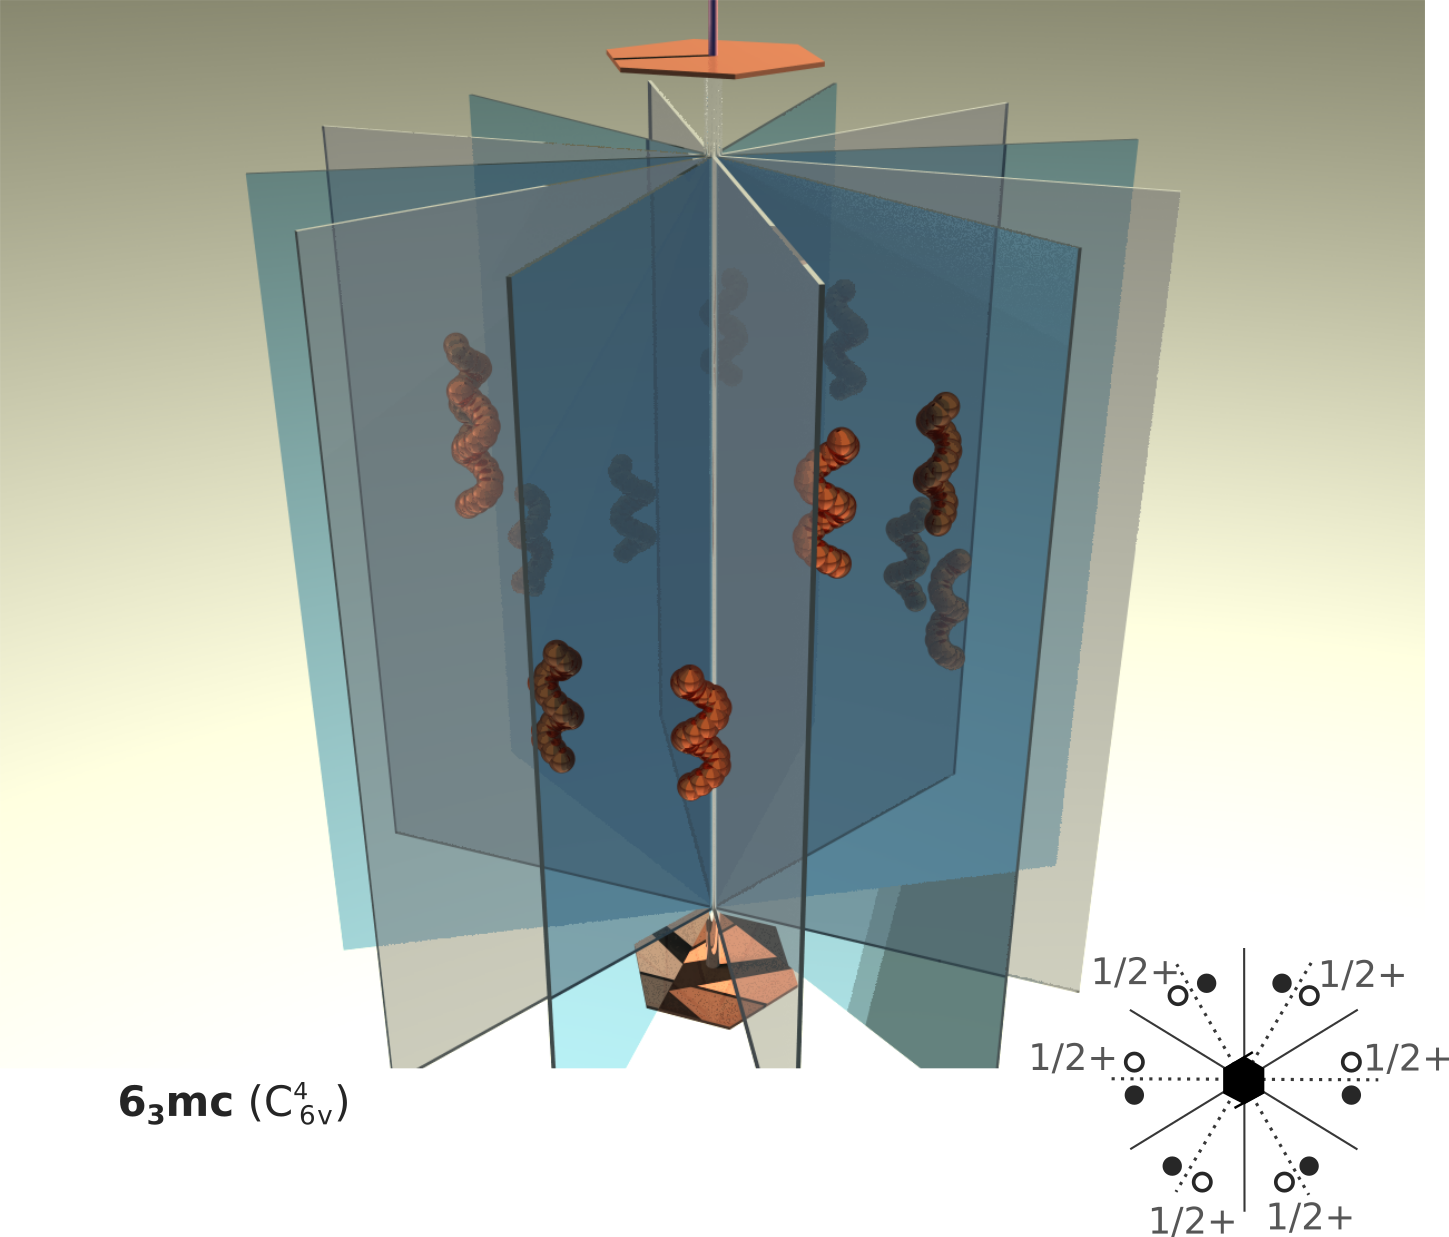
\includegraphics[width=1.\linewidth]{Figures/6_3mc.png}
\caption{Graphical 3D representation of the $\mathbf{6_3mc}$ symmetry combination. Blue planes represent the mirror planes and the grey ones the glide planes. See Appendix~\ref{Chap:Symmetry} for discussion on squiggly objects. The 2D projection is shown in the bottom right corner. Filled circles indicate the object is in the plane of the drawing, open circles indicate the object is above the plane at the indicated height). Dotted lines represent a glide plane with translation normal to the drawing plane and solid lines are mirrors. }
\label{Fig:6_3mc}
\end{figure}


We talked in Appendix~\ref{Chap:Symmetry} about how one can determine the full symmetry of a space group by adding the point group operators to a compatible Bravais lattice. Indeed, the space group symbol itself is made up of the Bravais lattice information to which the point-group Hermann-Mauguin notation is added. Let us consider the space group $\mathbf{P6_3mc}$. If we start with the primitive hexagonal Bravais lattice $hP$ and add the $\mathbf{6mm}$ point group (see page~\pageref{subChap:pointGroup}) at every lattice point we obtain the $\mathbf{P6mm}$ space group. But we can generate a new group with a different symmetry if we replace the $\mathbf{6}$ symbol in the point group with a $\mathsf{6_3}$ screw axis operation (see page~\pageref{sec:screw}) and the second $\mathbf{m}$ with a glide plane $\mathsf{c}$ in the direction of basis vector $\mathbf{c}$. The resulting symmetry group, $\mathbf{6_3mc}$, is shown in Fig.~\ref{Fig:6_3mc}. The blue planes are the mirror planes with normal \hkl{10.0} and, in between them, the grey planes represent the glide planes with normal \hkl{12.0}. 


As before, the generating files can be found in \texttt{6\_3mcPNG.ray} for the \textit{*.png} image and \texttt{6\_3mcGIF.ray} for the \textit{*.gif} animation. 


Note that this combination does not make up a point group as it does not present unique symmetry. However, when adding the $\mathbf{6_3mc}$ symmetry at the lattice points on a hexagonal primitive Bravais lattice it generate the brand new space group $\mathbf{P6_3mc}$. This is illustrated in Fig.~\ref{Fig:P63mc}, where the last image is taken from the \textit{Tables} and shows the top view projection of the symmetry operators of this space group. 

\begin{figure}
    \centering
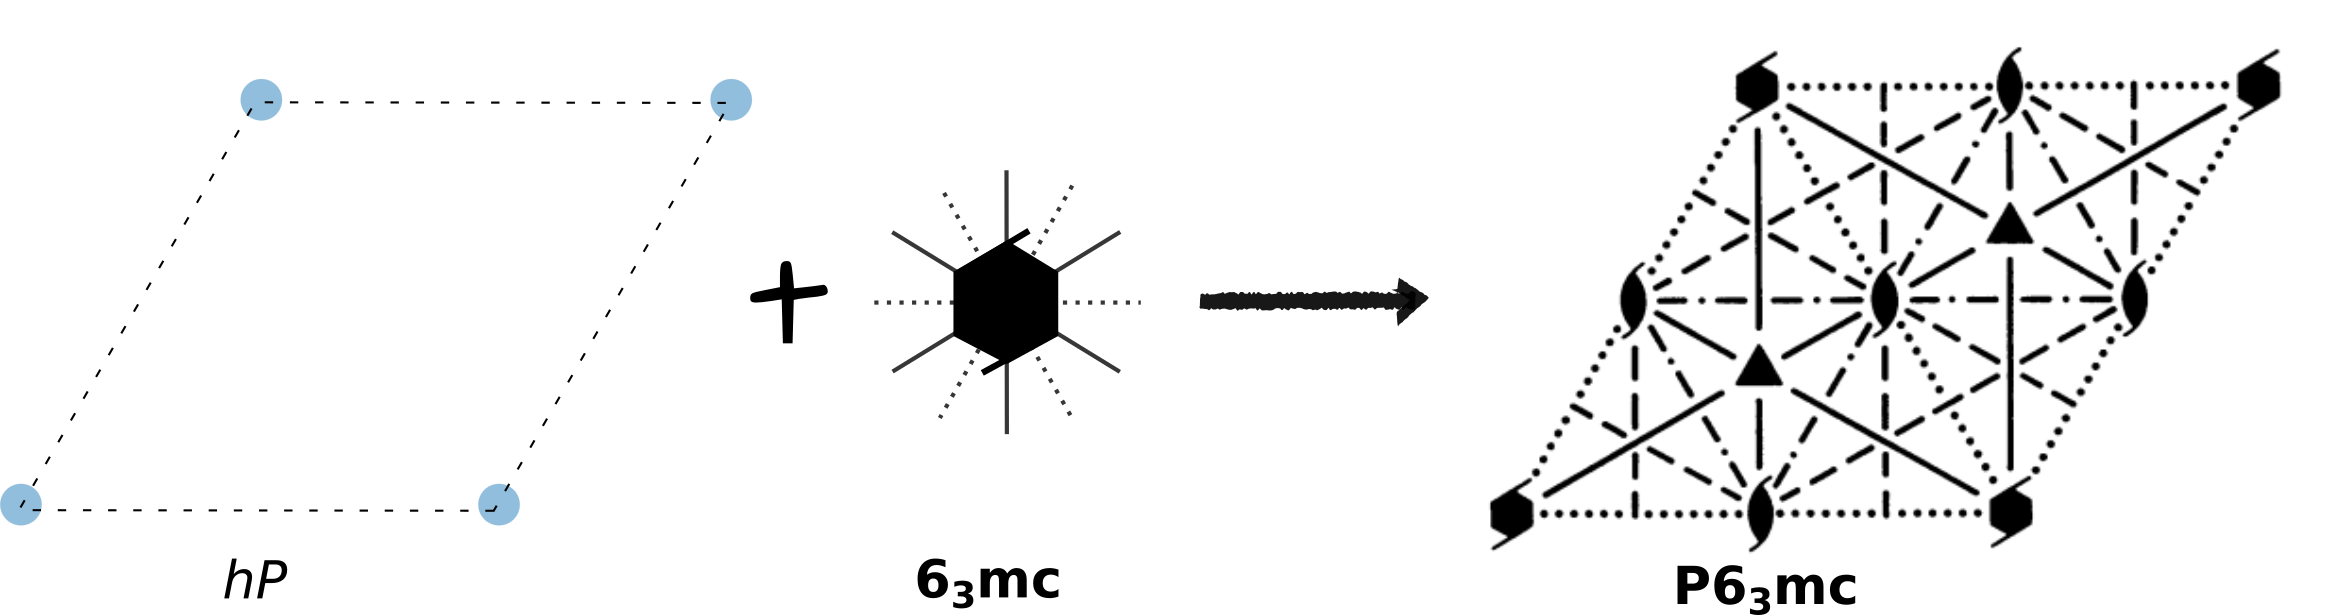
\includegraphics[width=0.9\linewidth]{Figures/spaceGroup.png}
\caption{Top view construction of space group $\mathbf{P6_3mc}$ from the Bravais lattice $hP$ combined with the symmetry combination $\mathbf{6_3mc}$. [Right image taken taken from ref.~\cite{IntTableCrysA}.]}
\label{Fig:P63mc}
\end{figure}

\begin{table}
\caption{The $\mathbf{P6_3mc}$ space group with its corresponding number and crystallographic point group.}
\label{Table:wurtziteSpace}
\centering
\begin{tabular}{l c c c }
\toprule
\tabhead{Space group \#} & \tabhead{Point group} & \tabhead{Space group symbol}  \\
\midrule
 186 & $\mathbf{6mm}$ & $\mathbf{P6_3mc}$ \\
\bottomrule
\end{tabular}
\end{table}

One can find the corresponding point group of a space group containing glide planes or screw axes (non-symmorphic) by simply replacing the glide planes by mirrors and the screw axes by regular rotations. We show in Table~\ref{Table:wurtziteSpace} the corresponding crystallographic point group together with the space group number as it is indexed in the \textit{ International Tables for Crystallography}. The important difference to keep in mind when comparing the space group $\mathbf{P6_3mc}$ with the corresponding point group $\mathbf{6mm}$ is that the space group symmetry includes translational vectors. And in this case, we are not only talking about the Bravais lattice translational vectors, but also about symmetry operators of second kind, like screw and glide, that include translation. In mathematical language, this means that the point symmetry matrices $\mathsf{D^{(x)}}$ are not sufficient for describing the symmetry of the the space group and we must turn to the $4\times 4$ matrices, $\mathcalboondox{W}$, which contain translation information as well. We showed on page~\pageref{eq:Wdef} (Eq.~\ref{eq:Wdef}) how to write these matrices using the Seitz symbols: $\mathcalboondox{W}=(\mathsf{D}|\boldsymbol{\tau})$.
The values of the relevant matrices $\mathsf{D^{x}}$ are given explicitly in Appendix~\ref{Chap:Symmetry}.


In Appendix~\ref{Chap:Symmetry} we derived the 12 symmetry operations of this space group. We also mentioned that these can also be found as list in the \textit{Tables}. We will need these symmetry operations in order to determine the equivalent positions of an atom in the unit cell, \ie for a given atom position apply all symmetry operations of the space group to this position and note all unique new coordinates inside the unit cell.

With the help of Appendix~\ref{Chap:Symmetry} we can read all the symmetry operations symbols in the right image of Fig.~\ref{Fig:P63mc}. Especially we can recognise the 4 group generators listed in the \textit{Tables} (shown on page~\pageref{Fig:ITC}). Table~\ref{Table:generators} describes these generators and points to the Appendix pages were they are discussed. The table also gives us the matrices we need to apply to a position $(x, y, z )$ when looking its symmetry equivalent places in the unit cell. 



\begin{table}
\caption{List of generators for wurtzite crystal structure.}
\label{Table:generators}
\centering
\begin{tabular}{c l l c l }
\toprule
\tabhead{\thead{Operation \# \\ in \textit{Tables}}} & \tabhead{ \thead{Representation \\in \textit{Tables}}} & \tabhead{Description (page discussed)} & \tabhead{Graphical} & \tabhead{Seitz symbol }  \\
\midrule
 (1) & 1                            & identity                                   &         & $(\mathsf{D^{(a)}}|\mathbf{0})$  \\
 (2) & $3^+ \, 0,0,z$               & 3 fold rotation around \hkl[001] (\pageref{sec:pureRot})       & \cry{3} & $(\mathsf{D^{(n)}}|\mathbf{0})$  \\
 (4) & $2(0,0,\frac{1}{2})\, 0,0,z$ & $\mathsf{2_1}$ screw axis around \hkl[001]  (\pageref{sec:screw})& \cry{21} & $(\mathsf{D^{(b)}}|\boldsymbol{\tau}_{(0,0,1/2)})$  \\
 (7) & $m\, x, \bar{x}, z$          & \hkl(110) mirror plane  (\pageref{sec:pureRefl})                    & \rule[1pt]{0.3in}{1.5pt} & $(\mathsf{D^{(k)}}|\mathbf{0})$  \\
\bottomrule
\end{tabular}
\end{table}



%From the \textit{Tables} we learned a few important properties of this space group that we will need to use in the diffraction models. 






\subsection{Wurtzite crystal structure}
It is customary to describe a crystal structure by its space group, lattice parameters and atom positions in the asymmetric unit cell. We have covered group symmetries so far, and it is therefore time to place atoms on the lattice. 

Unfortunately, some ambiguity about the positions of the wurtzite atoms in the unit cell exists. Figure~\ref{Fig:wurtzite} a) shows the common representation of a wurtzite unit cell. This is a didactically useful way to visualise the hexagonal close packing (hcp) structure that wurtzite exhibits. For this unit cell we can place an atom at $(0,0,0)$ and another, identical one at $(1/3, 2/3, 1/2)$. A pair of atoms of a  different species can then be displaced by a value $x$ in the \textbf{c}-$axis$ direction with respect to the first two. For the perfect wurtzite structure $x=3/8$. This unit cell will have the translational symmetry of the primitive hexagonal Bravais lattice, $hP$. 

\begin{figure}
    \centering
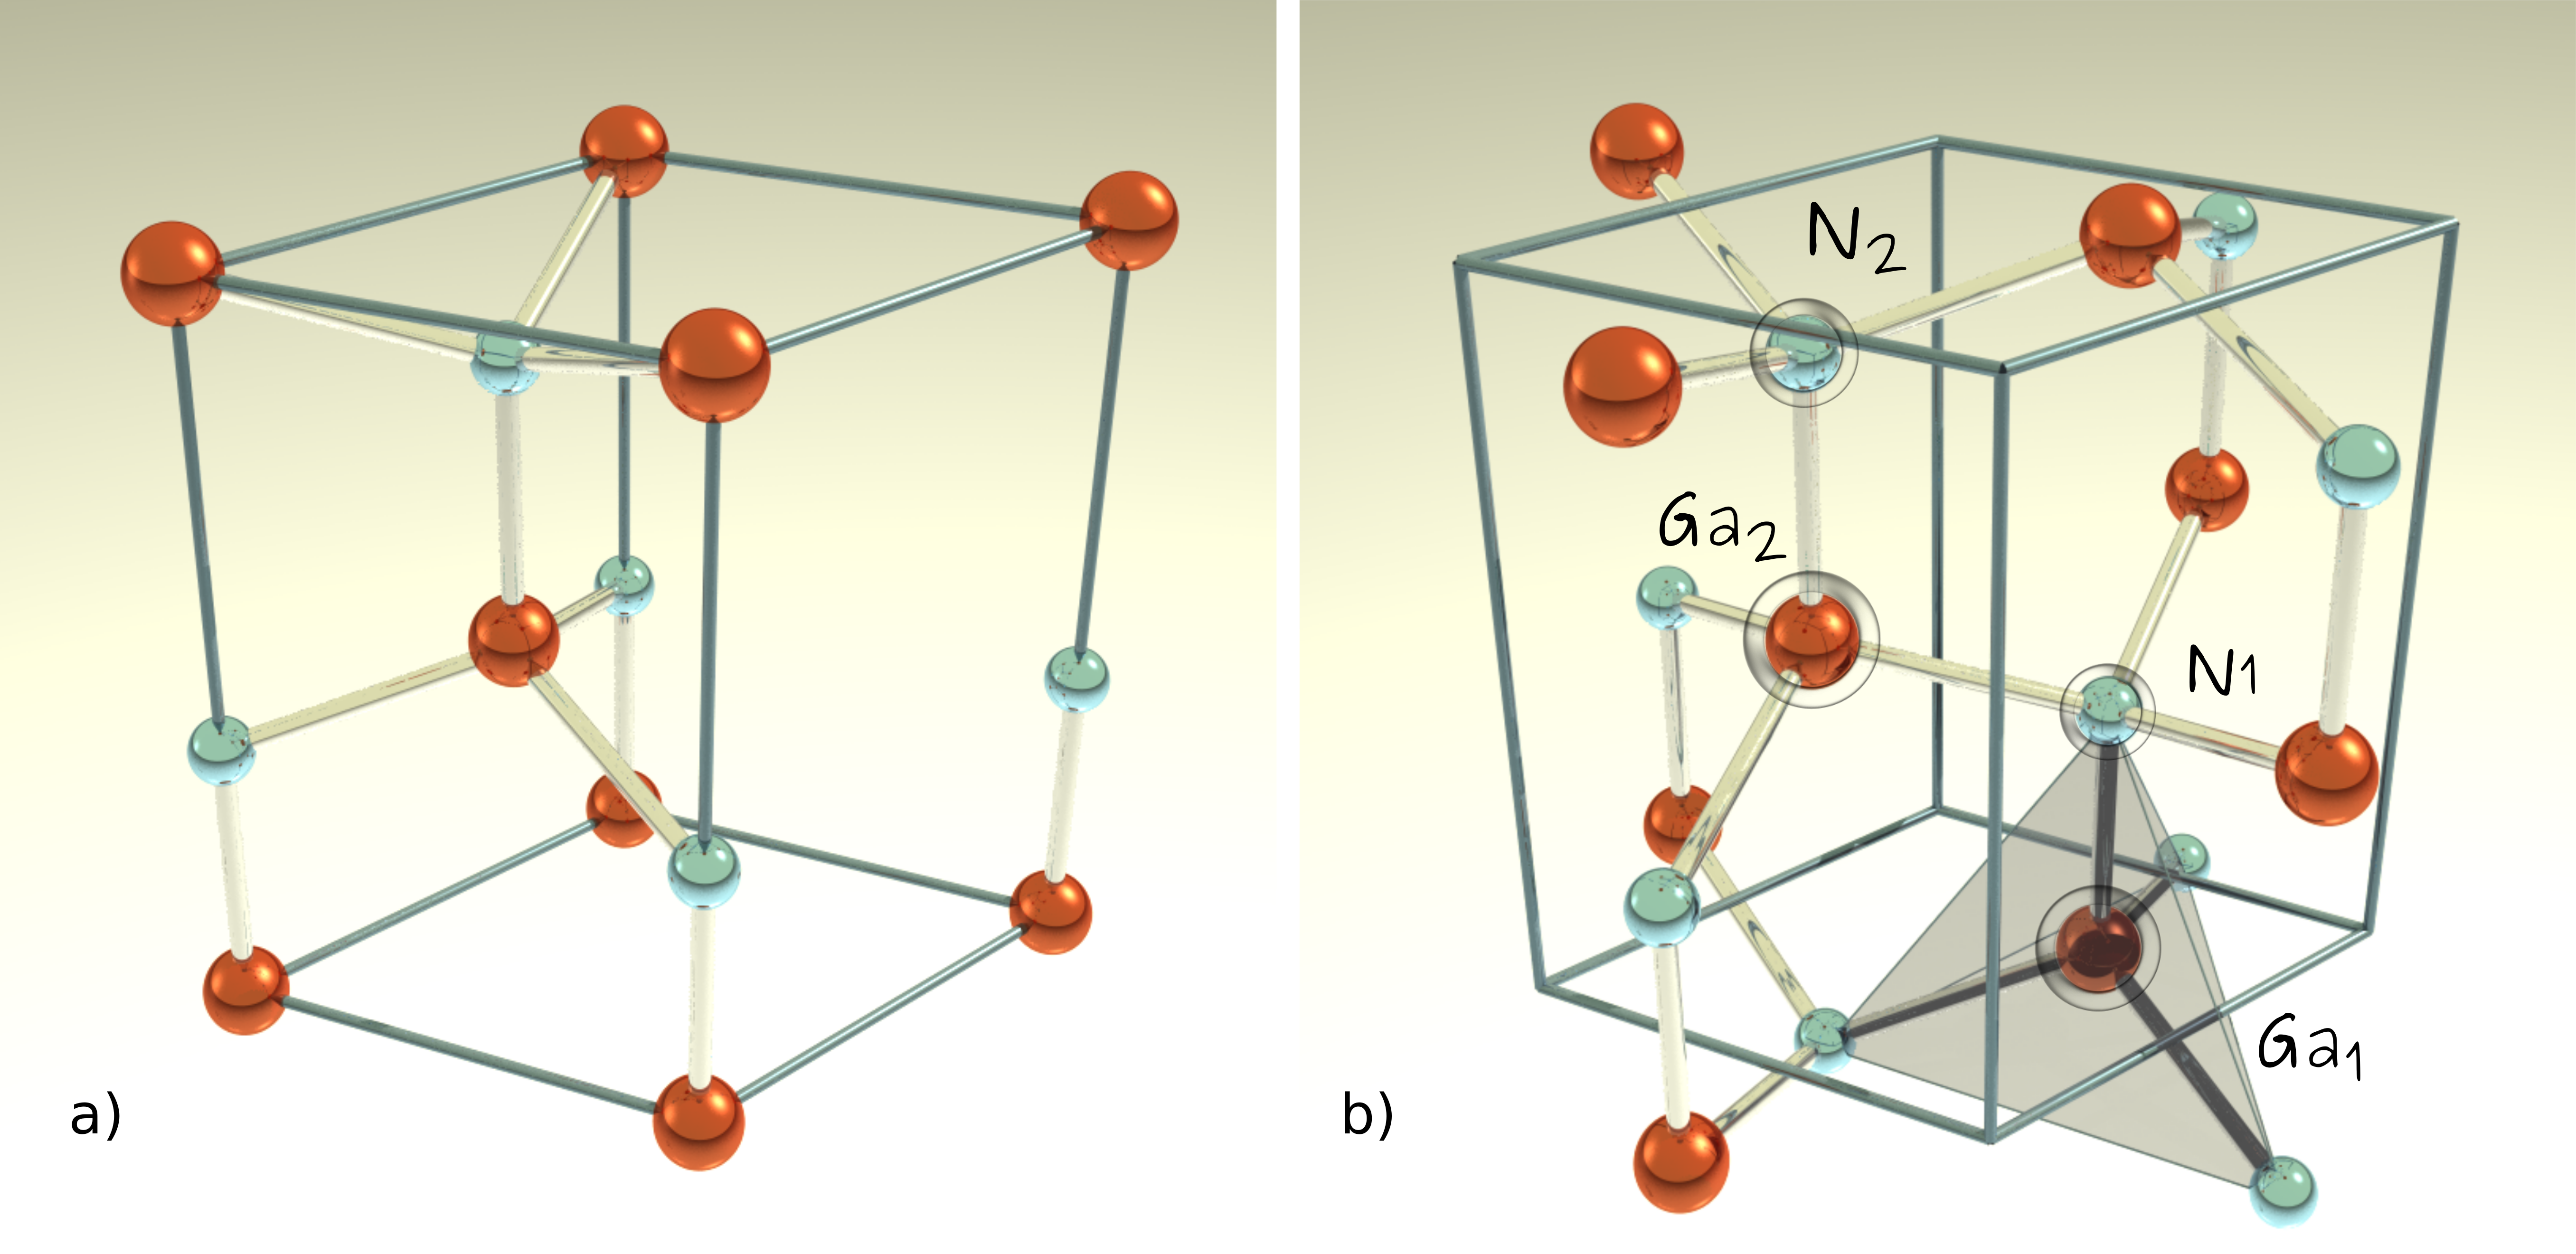
\includegraphics[width=1.0\linewidth]{Figures/wurtzite_compare.png}
\caption{3D render of: a) hexagonal unit cell representation of hcp structure of wurtzite, not respecting group symmetry; b)  wurtzite crystal structure  hexagonal primitive cell ($hP$) enclosed by blue edges and the tetrahedral asymmetric unit cell enclosed by glass faces. The 4 highlighted atoms are the ones contained by the primitive unit cell.}
\label{Fig:wurtzite}
\end{figure}


Nevertheless, this representation does not carry the symmetry of the space group $\mathbf{P6_3mc}$ to which wurtzite belongs. Figure~\ref{Fig:wurtzite} b), on the other hand, shows the unit cell of a $\mathbf{P6_3mc}$ space group structure exhibiting the full symmetry of this group.  The atoms are now placed at the $2b$ Wyckoff positions given as fractional coordinates of the basis vectors:
\begin{align}
\label{eq:positionGa1}
    \text{Ga}_1 & :(1/3,\, 2/3, \, z=0)\\
\label{eq:positionN1}
    \text{N}_1  & :(1/3,\, 2/3, \, z+x=0+x)
\end{align}
where $x=3/8$ for the ideal wurtzite structure as before. 

These two atoms are enough to define the asymmetric unit cell highlighted here by the tetrahedrally  shaped grey box. Looking closer at  the symmetry of the asymmetric cell we can recognise the glide, or, equivalently, screw symmetry we have seen in the $\mathbf{6_3mc}$ symmetry group render in Fig.~\ref{Fig:6_3mc}. The mirror planes pass through the tetrahedral cells indicating the unit cell exhibits mirror symmetry, \ie we replace the pair of squiggly orange objects with the asymmetric unit cell. Any atom or group of atoms in the unit cell in ~\ref{Fig:wurtzite}~b) will satisfy all the symmetry operations of the space group shown in Fig.~\ref{Fig:P63mc}. Note that this is not the case for the unit cell in a).

The positions of the other atoms in the fundamental, hexagonal prism unit cell shown in  Fig.~\ref{Fig:6_3mc}~b) can be determined by applying the list of 12 symmetry operations of the space group to the positions inside the asymmetric unit cell given above. It turns out that we only need one operation to generate two new positions inside the unit cell. A number of operations can produce the two new positions, for instance the $\mathsf{2_1}$ screw operation with entry (4) in Table~\ref{Table:generators} with the origin the middle of the cell or a  $\mathsf{6_3}$ screw with the origin at the origin of the cell. 

\begin{align}
\label{eq:positionGa2}
    \text{Ga}_2 & :\mathcalboondox{W}_\text{\cry{21}} \text{Ga}_1 =(2/3,\, 1/3, \, z'=1/2)\\
\label{eq:positionN2}
    \text{N}_2  & :\mathcalboondox{W}_\text{\cry{21}} \text{N}_1 =(2/3,\, 1/3, \, z'+x=1/2+x)
\end{align}
where $x=3/8$ for the ideal wurtzite structure.
The  hexagonal unit cell is populated by the same 4 atoms as the one in Fig.~\ref{Fig:wurtzite}~a). The two cells can generate the same structure, a) by translation only and b) by applying the generators of the space group. We will be using in this work exclusively the latter representation of this cell since the diffraction properties we are interested in are the result of the group symmetry.

The files used to render the $^*.png$ and $^*.gif$ versions of the images shown in this section are: \texttt{wurtzite\_commonGIF.ray} for the first version of the cell shown in a) and \texttt{wurtzite\_cellGIF.ray} for the latter.







\subsection{Nitrides lattice parameters}
Finally, the lattice parameters can be calculated from first principles and/or from diffraction experiments. I am showing in Table~\ref{Table:wurtziteLatPar} the currently accepted lattice parameters for the three wurtzite systems we tackled in this work. The last entry shows the volume of the fundamental cell calculated using Eq.~\ref{eq:UnitCellVolume} derived on page~\pageref{eq:UnitCellVolume}.


\begin{table}[h]
\caption{Lattice parameters and unit cell volume, $\Omega$, for some common nitrides with wurtzite crystal structure.}
\label{Table:wurtziteLatPar}
\centering
\begin{tabular}{l c c c }
\toprule
\tabhead{Wurtzite compound} & \tabhead{a [\si{\angstrom]}} & \tabhead{c [\si{\angstrom]}} & \tabhead{$\Omega$ [\si{\angstrom^3]}} \\
\midrule
 AlN~\cite{Goldberg01} & 3.11 & 4.98 & 41.71 \\
 GaN~\cite{Leszczynski94} & 3.19 & 5.19 & 45.74\\
 InN~\cite{Zubrilov01} & 3.53 & 5.70 & 61.51\\
\bottomrule
\end{tabular}
\end{table}
 
\pagebreak

\section{Electron scattering}


Before we can talk about diffraction we need to address the phenomena of scattering. Classically, the collision of particles is fully defined by their velocities and interaction parameters. However, high energy electrons are quantum mechanical objects. The notion of defined path for particles with known velocity is meaningless in the quantum mechanical world. Instead, we are interested in defining the probability that, as a result of the collision, the particle will deviate by a given angle. We call this \textit{scattering}.

Electrons are small charged particles that will suffer multiple scattering events even in thin samples in contrast to X-ray and neutron interactions with matter. Electron scattering in a solid is a complex multi dimensional problem. For practical considerations it is common to classify the interaction of electrons with a crystal in two distinct processes:
\begin{itemize}
\item \textit{Elastic scattering}, defined as a process which does not change the state of the crystal. Mostly made up by interactions with the nucleus: Rutherford scattering taking into account just Coulomb forces between the charged electron and the nucleus. This account for most of the angular scattering.


\item \textit{Inelastic scattering}, defined as the process in which the state of the crystal is modified by the interaction. Important contribution here is made by the electron-electron scattering which cause the incident beam electron to loose small amounts of energy but cause relatively little angular deflections.
\end{itemize}


%-----------------------------------
%	Scattering, see Joy and MC modelling
%-----------------------------------
\pagebreak
\subsection{Elastic scattering }

Elastic collision reduces, in the quantum mechanical world, to the interaction of a free particle interacting with a fixed potential field $U(\mathbf{r})$.


\paragraph{Rutherford scattering}

\subsection{Inelastic scattering }

\paragraph{Bethe's equation}



\pagebreak
\section{The scanning electron microscope}

% microscopy
The phenomena described in the previous section occur at a scale too small to be measured by the naked eye. Luckily,  development of science had brought us two main extension  to the range of scales we can study. Interestingly, both these aids can be traced back to a \nth{17} century event: the development of glass lenses used in spectacles, and both are governed by the same optics laws. On one hand the telescope brings very distant object closer and is optimised to collect as much light as possible and, on the other, the microscope makes very close close objects appear many times larger. 

While modern light microscopes can showcase a magnification of about $2000\times$, their resolution is limited by Abbe's equation. One way around it is to use imaging particles with smaller wavelength like electrons.   

%relativistic correction
Let us shortly address relativistic corrections for electrons used in electron microscopy. The de Broglie equation for the relativistic electron  wavelength, $\lambda$, can be written in terms of the accelerating voltage $V$ (equation 2.4 in \cite{goodhew88}) as:
\begin{equation}
    \lambda = \sqrt{\frac{150}{V + 10^{-6}\, V^2}} \,\, [\si{\angstrom}]
\end{equation}
where the second term is the correction term and becomes important for voltages grater than $20$ \si{\kilo \electronvolt} as we can see in Table~\ref{Table:wavelength}.

For SEM applications discussed in this work we will focus on $20$ \si{\kilo \electronvolt} incident electrons, and discard, quite acceptably, relativistic effects. 

\begin{table}
\caption{Corrected and uncorrected electron wavelengths for voltages used in  electron microscopy.}
\label{Table:wavelength}
\vspace{-0.4cm}
\centering
\begin{longtable}{l c c c}\toprule
             \multirow{2}{*}{\tabhead{Voltage [\si{\kilo \electronvolt}] }} &  \multirow{2}{*}{\tabhead{Lorentz factor $\gamma$} \hspace{0.4cm}}  & \multicolumn{2}{c}{\tabhead{Wavelength  $\lambda$ [\si{\angstrom}]}}\\ \cmidrule{3-4}
              &  &\tabhead{Uncorrected}        &  \tabhead{Corrected}  \\ \midrule
20   & 1.04  & 0.086 & 0.086  \\
100  & 1.20  & 0.039 & 0.037  \\
1000 & 2.93  & 0.012 & 0.009  \\
\bottomrule
\end{longtable}
\end{table}


\noindent\begin{minipage}{0.5\textwidth}
Another key difference between the SEM and the TEM is the operation method. Excellent detailed description of the scanning electron microscope can be found in ref.~\cite{Hearle72} and~\cite{Reimer13}.  For our purposes the simplified schematics in Figure~\ref{Fig:sillySEM} will be enough. As the electron beam is scanned in a raster manner over the area of interest on a tilted sample, the detector collects one pixel worth of information at a time and the entire image is shown on a display when the scan ends.  
\end{minipage}%
\begin{minipage}{0.5\textwidth}
    \centering
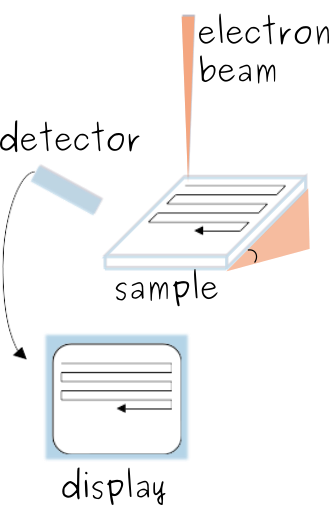
\includegraphics[width=0.5\linewidth]{Figures/sillySEM.png}
\captionsetup{width=.7\linewidth}
\captionof{figure}{SEM schematics.}
\label{Fig:sillySEM}
\end{minipage}

\vspace{0.4cm}

There is a variety of signals that the SEM can measure. Traditionally, secondary electrons are collected for excellent surface imaging applications as well as information about density change across the sample. Optical information can also be inferred by collecting the light emitted by excited atoms in a technique known as cathodoluminescence. However, we will be concerned with none of these signals. The information we will be interested in this work will be made up of electrons undergoing diffraction in the crystal and being backscattered towards the detector. 

% TILT
The tilt of the sample in the SEM ensures that  enough electrons reach the detector. It also makes the geometry of diffraction very different from that in the TEM. The sample's z-direction in the SEM is not the same as the beam direction which is the case for the TEM sample geometry. This means that if we are to use the diffraction models developed for TEM, they must be generalised for the sample tilt.  More about his in the next chapter. 

The references above discuss the electron optics as well and we will not delve on it here. We will however mention that the tilt of the sample affects the ``squareness'' of the scanned area. The trapezoidal area scanned will produce a distorter image, which can be corrected to some degree using the tilt correction function (see page 50 in ref.~\cite{SEMbooklet} for tilt correction artefacts). The tilt can also change the shape of the beam on the sample which not only affects the imaging but also the diffraction interaction volume. 